%*******************************************************************************
%****************************** Fourth Chapter *********************************
%*******************************************************************************


\chapter{GEANT4 Simulation}\label{chp:GEANT4Simulation}
\ifpdf
    \graphicspath{{Chapter4/Figs/Raster/}{Chapter4/Figs/PDF/}{Chapter4/Figs/}}
\else
    \graphicspath{{Chapter4/Figs/Vector/}{Chapter4/Figs/}}
\fi

\section{GEANT4 Overview}\label{sec:GEANT4Simulation_g4Overview}
The VIDARR detector is represented in a GEANT4 simulation which is a provident physics simulation package. According to the GEANT4 collaboration GEANT4 ``covers a comprehensive range including electromagnetic, hadronic and optical processes and a large set of long-lived particles materials and elements over a wide energy range starting in some cases from 250\,eV and extending in others to the TeV range'' \cite{Agostinelli:2002hh}. Considering that the energy range for IBD is $\sim$ 1.8\,MeV -- $\sim$ 8.5\,MeV \cite{Mueller_2011} this simulation package meets the needs of the VIDARR collaboration. IBD produces e$^+$ and neutrons (see equation \ref{inverse_beta_decay}) whilst the simulation of e$^+$ is reasonably straight forward the simulation of the neutrons is more complex. This is due to the gadolinium sulphate sheets that capture the neutrons and emit an 8\,MeV $\gamma$ cascade. The Gadolinium cascade is hard to model accurately due to the high energies and number of nucleons involved ($>$ 150).
\\\\The simulation has several distinct modes: cosmic $\mu$, Dark noise, background, and inverse $\beta$ decay. The cosmic model has a realistic distribution based on the Cosmic Ray Shower Library (CRY) \cite{ieee_cry_2007} and a cosmic hemisphere distribution. The cosmic hemisphere distribution is used to determine any bias in the comic tracker which reconstructs cosmic $\mu$ events. In all other cases, the realistic cosmic distribution is used when simulating cosmic $\mu$. The background distributions are random uniform distributions from 0 -- 10\,MeV simulating which cover $p$,$\bar{p}$,$\pi^+$,$\pi^-$,$e^-$,$e^+$, $\alpha$,$\bar{\alpha}$,$n$. IBD is approximated by simulating a positron and a neutron simultaneously the positron energy is a flat distribution between 0\,MeV -- 10\,MeV the neutron takes $\sim$ 50\,$\mu$s to be absorbed (see figure \ref{fig:delayedIbdTimes}) . The range 0\,MeV -- 10\,MeV is used instead of 1.8\,MeV -- 8.5\,MeV for more robust fitting and identification of edge cases.
\\\\An example of a simulated IBD event can be seen in figure \ref{fig:simultaedIbdEvent}, the simulation produces a e$^+$ and neutron simultaneously it does not simulate the $\bar{\nu_e}$ interaction with matter. This is not a major constraint as this is the signal that the detector measures but it does mean that the $\bar{\nu_e}$ rate is not modelled by the simulation. The times for the generated neutron to complete its random walk through the detector + the time taken for the Gadolinium sheets in-between the segments to absorb the neutron + the time taken for the cascade to occur is shown in figure \ref{fig:delayedIbdTimes}. It is possible for the neutron absorption to take up to 100 $\mu$s when simulating a kinetic energy of 10\,keV. A kinetic energy of 10\,keV is a reasonable assumption when considering the work of Vogel and Beacom \cite{Vogel_1999}. 


\begin{figure}[!h]
\centering
\begin{minipage}{.45\textwidth}
  \centering
  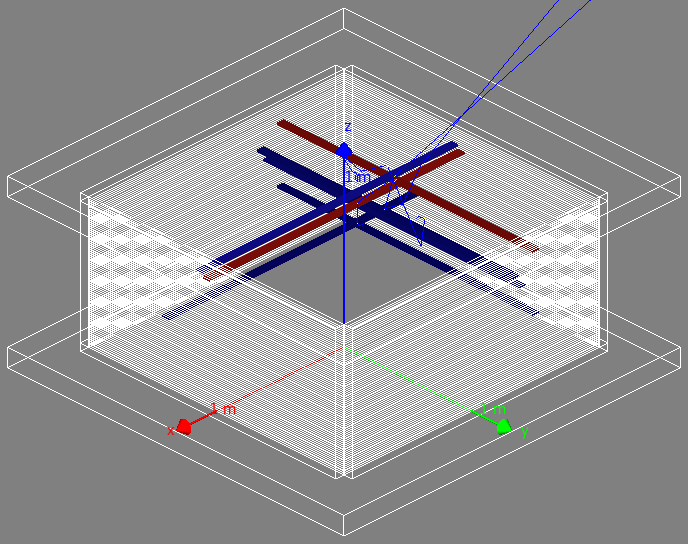
\includegraphics[width=\linewidth]{Chapter4/Figs/Raster/simultaedIbdEvent.png}
  \captionof{figure}{A simulated inverse $\beta$ decay event in GEANT4 in the upgraded detector with 70 layers and shielding around the outside of the detector. The delayed component is shown in blue and the prompt component is shown in red. The delayed component hits more bars than the prompt component.} 
  \label{fig:simultaedIbdEvent}
\end{minipage}%
\qquad
\begin{minipage}{.45\textwidth}
  \centering
  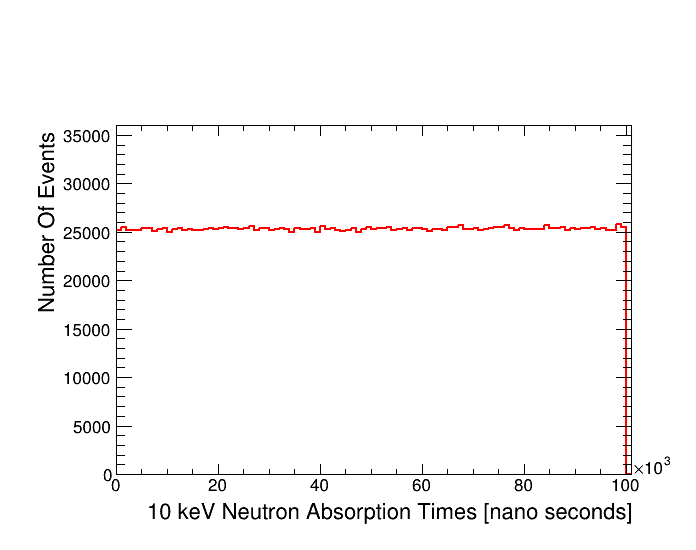
\includegraphics[width=\linewidth]{Chapter4/Figs/neutron10KeVAbsoptionTimes.png} 
  \captionof{figure}{The time taken for the neutron from the simulated $\bar{\nu_e}$ inverse $\beta$ decay event to be thermalised and be absorbed by the Gadolinium sheets in the simulated VIDARR detector. Assuming a kinetic energy of 10KeV for the neutonrs leading to a flat distribution from 0 -- 10$^5$ ns (0-100\,$\mu$s).}
  \label{fig:delayedIbdTimes}
\end{minipage}
\end{figure}

\section{Modelling The Mass Increase}
The number of layers in the RMon detector was 49 out of a possible 70 the upgrade will therefore add $\sim$ 43\,\% additional mass into the detector compared to the RMon detector. In reality, out of a possible 1862 channels in RMon, only 1793 were instrumented due to limitations in securing enough parts. Never the less the simulation will focus on the theoretical maximum number of bars in both cases for the sake of simplicity. As can be seen from figure \ref{fig:prototypeMeasumentFlux} there is an expectation of $\sim$ 200 $\Bar{\nu_e}$ a day and so from the upgraded detector, it is reasonable to assume a rate of $\sim$ 300 $\Bar{\nu_e}$ a day with the additional mass. But in addition, the quality of each event will also improve as more of the energy from the 8\,MeV $\gamma$ cascade is kept within the bounds of the detector. The amount of energy deposited in the detector will be considered the ``containment'' of the cascade where containment of 100\,\% would mean 100\,\% of the energy is deposited in the detector. And as figure \ref{fig:containment_comparison} shows the quality of the containment improves with more mass. %In figure \ref{fig:containment_comparison} it can be seen that the quality of the containment increases when the additional mass has been added. 

\begin{figure}[!h]
 \centering
 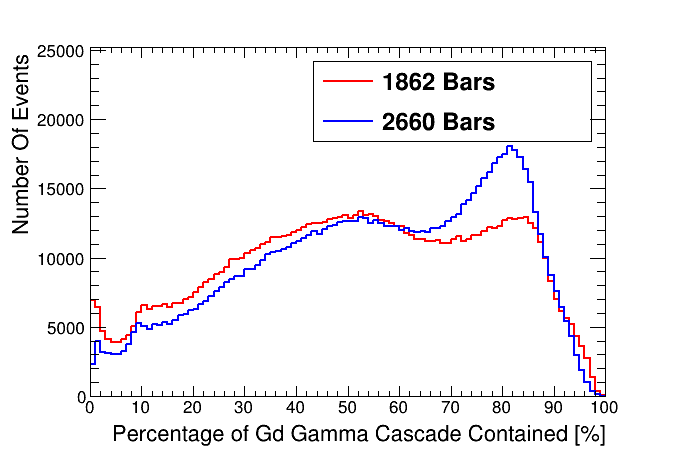
\includegraphics[width=0.7\linewidth]{Chapter4/Figs/cascadeContainmentCompare.png}
 \captionof{figure}{Percentage of neutron induced Gd $\gamma$ cascade deposited energy to $\gamma$ cascade generated energy for 1862 bar (49 layers) and 2660 bars (70 layers). The quality of the events improves with the taller detector as expected. Cascade containment $\leq$ 0.1\,\% is treated as 0\,\%. }
 \label{fig:containment_comparison}
\end{figure} 

When simulating e$^-$s and e$^+$s with 0\,MeV -- 10\,MeV kinetic energy the amount of energy contained inside is $\sim$ 100\,\% but slowly decreases as the energy increases. The amount of energy generated (E$_\textrm{{gen}}$) versus the energy deposited  (E$_\textrm{{Dep}}$) for these two particles is shown in figure \ref{fig:recon_gen_ele_pos} contains the energy of charged particles, even small mass particles such as e$^-$ and e$^+$. Then e$^+$ particles are simulated from 1\,MeV -- 10\,MeV to determine efficiencies in figure \ref{fig:2000_3000_p_secs} for both 1862 bars (figure \ref{subFig:2000_p_sec}) and 2660 bars (figure \ref{subFig:3000_p_sec}) above a 0.1\,MeV threshold. In both cases the efficiency doesn't fall below 99\,\% for positrons this is due to the fact that positrons typically don't escape the detector without depositing $>$ 0.1\,MeV in at least a single bar. As such e$^+$ efficiencies don't significantly improve with the mass increase but are extremely high regardless.  

\begin{figure}[!h]
 \centering
 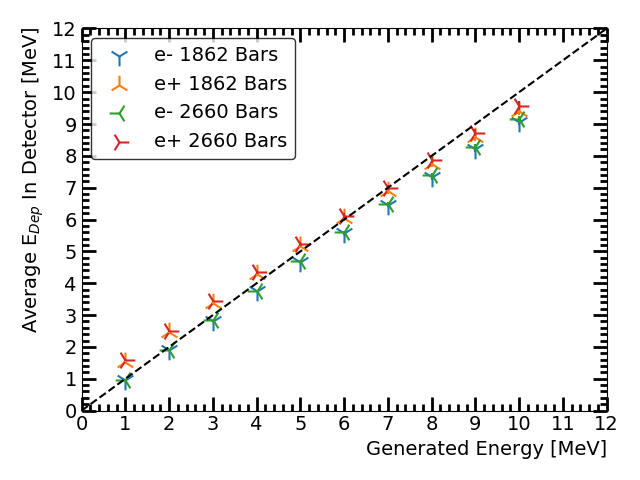
\includegraphics[width=0.7\linewidth]{Chapter4/Figs/summedVsTruth_1862_2660_e-e+_eBars_Adjusted.png}
 \captionof{figure}{Energy response of the simulated detector for both electrons and positrons in the full detector in comparison to E$_\textrm{{dep}}$ = E$_\textrm{{gen}}$. The positron's annihilation $\gamma$s causes E$_\textrm{{dep}}$ $>$ E$_\textrm{{dep}}$ at low generated energies. Generated energy has no error. The number of Generated events per point is 10$^5$ Errors for E$_\textrm{{dep}}$ are determined by standard error on the mean and are small but are shown on this plot.}
 \label{fig:recon_gen_ele_pos}
\end{figure} 

\begin{figure}[!h]
\centering
\begin{subfigure}{.5\textwidth}
  \centering
  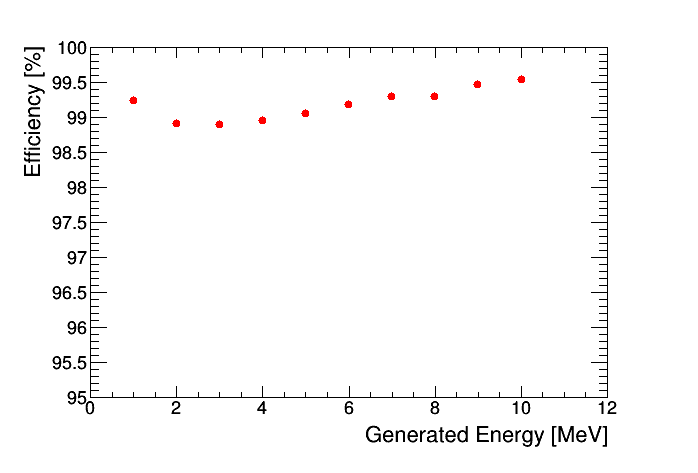
\includegraphics[width=\linewidth]{Chapter4/Figs/Raster/year1Plots/2000_1-10MeV_sec_p_spread_run.png}
  \captionsetup{width=.9\linewidth}
  \caption{}
  \label{subFig:2000_p_sec}
\end{subfigure}%
\begin{subfigure}{.5\textwidth}
  \centering
  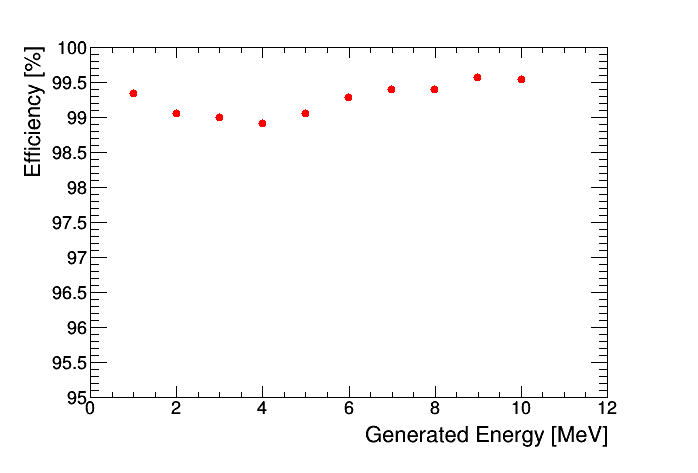
\includegraphics[width=\linewidth]{Chapter4/Figs/Raster/year1Plots/3000_1-10MeV_sec_p_spread_run.png}
  \captionsetup{width=.9\linewidth}
  \caption{}
  \label{subFig:3000_p_sec}
\end{subfigure}
\caption{Positron hit efficiencies for the original 1862 barred detector (see (a)) and the upgraded 2660 barred detector (see (b)) above a 0.1\,MeV threshold both have $\sim$ 99\,\% efficiencies are similar in both errors are too small to be shown Generated energy O $\sim$ $10^{-8}$ efficiency error O $\sim$ $10^{-3}$. }
\label{fig:2000_3000_p_secs}
\end{figure}

\section{Modelling $\mu$}
$\mu$ are high energy particles with high penetration. As a result atmospheric $\mu$ act as minimally ionising particles (MIPs), which means that the amount of energy deposited per cm ($dE/dx$) is largely independent of the generated energy in-between 100[MeV/$c$] -- 100[GeV/$c$] (see figure \ref{fig:pdg_MuonMomentumStopping}). Whilst figure \ref{fig:pdg_MuonMomentumStopping} shows many different effects and when they take effect for $\mu$ this figure only shows the effect incident on a copper surface. The detector is not comprised of Cu it is comprised of hydrocarbons, specifically polythene. By mass polythene is more C than H so by looking at the momentum ranges 0.1\,GeV/$c$ to 100\,GeV/$c$ in figure \ref{fig:pdg_dedx_gcm2} it is reasonable to assume a dE/dx of $\sim$ 2 g$^{-1}$ cm$^2$ for $\mu$ on C. 

\begin{figure}[!h]
 \centering
 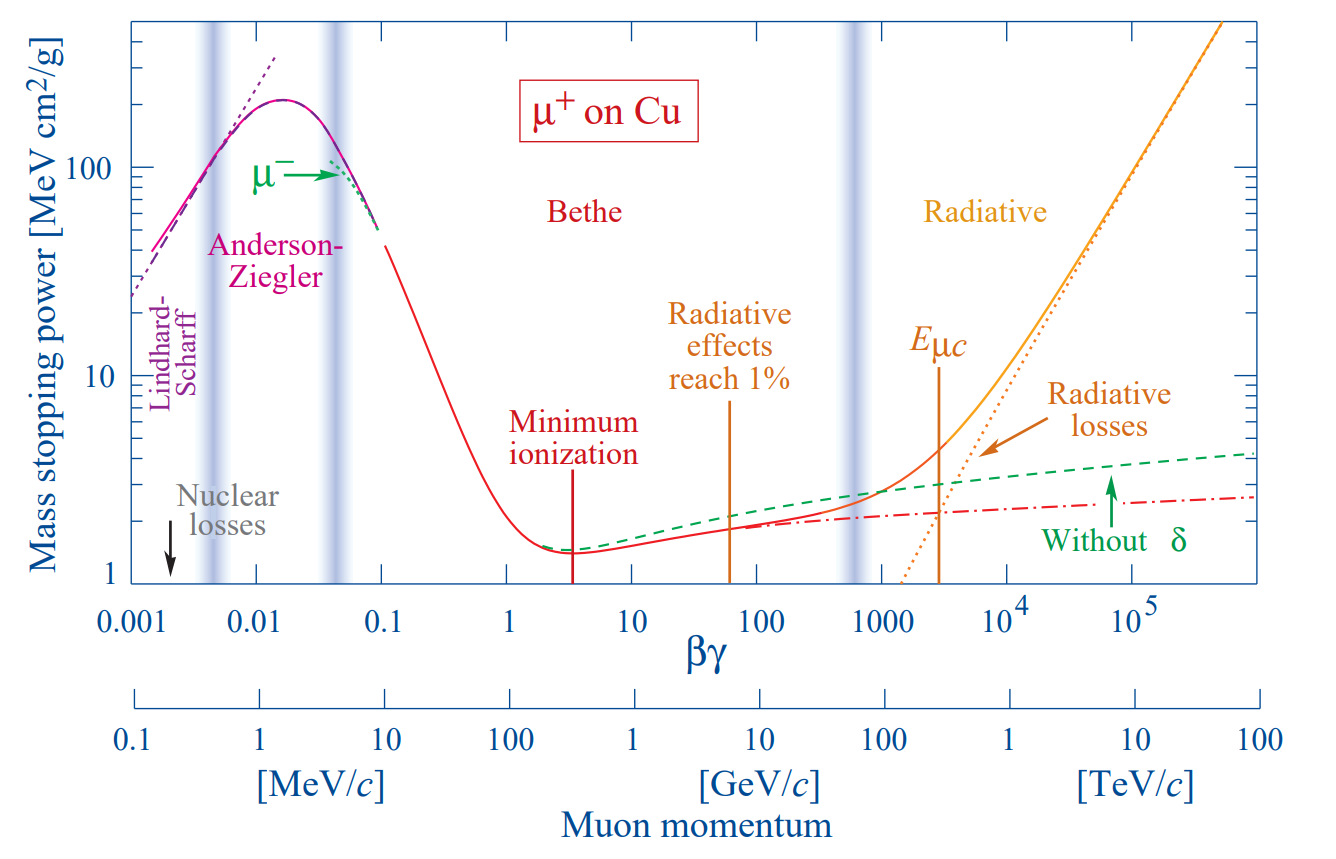
\includegraphics[width=0.7\linewidth]{Chapter4/Figs/Raster/pdg_MuonMomentumStopping.png}
 \captionof{figure}{Mass stopping power for positive $\mu$ in copper as a function of $\beta$ $\gamma$ = $\rho/Mc$ over nine orders of magnitude in momentum (12 orders of magnitude in kinetic energy). From \cite{Olive_2014}.} 
 \label{fig:pdg_MuonMomentumStopping}
\end{figure}

\begin{figure}[!h]
 \centering
 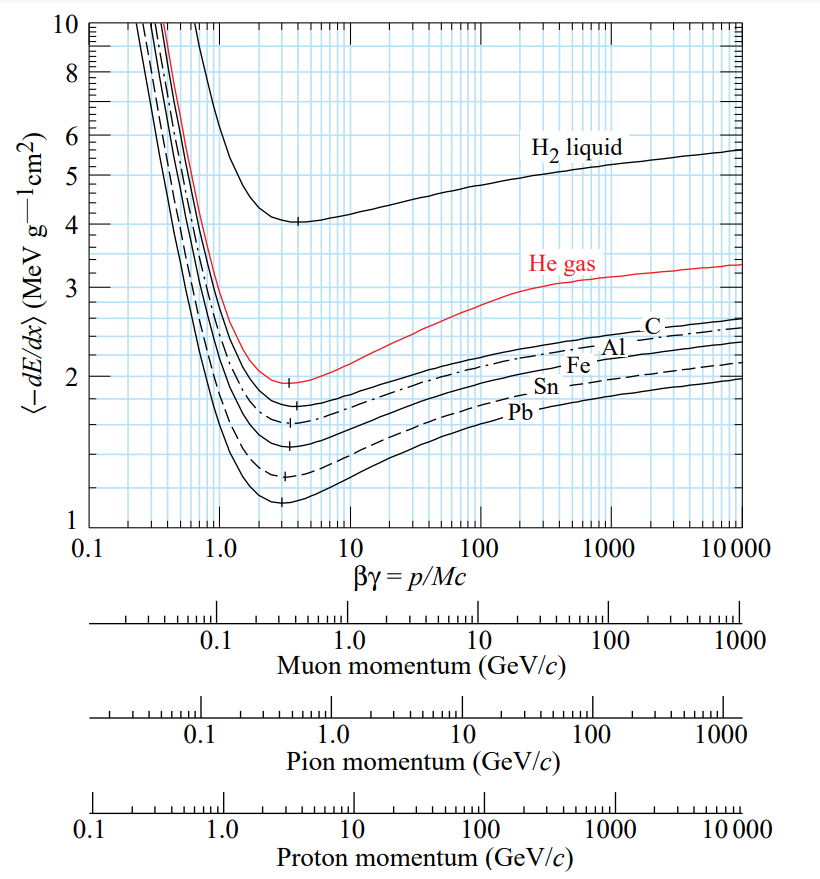
\includegraphics[width=0.7\linewidth]{Chapter4/Figs/Raster/pdg_dedx_gcm2.png}
 \captionof{figure}{Mean energy loss rate in liquid (bubble chamber) hydrogen, gaseous
helium, carbon, aluminium, iron, tin, and lead. Radiative effects, relevant for
$\mu$ and $\pi$, are not included. From \cite{Olive_2014}.} 
 \label{fig:pdg_dedx_gcm2}
\end{figure}

By simulating a single scintillating bar of dimensions 4\,cm $\times$ 152\,cm $\times$ 1\,cm (X,Y,Z) and firing a $\mu$ directly down in the Z plane it is possible to measure the $dE/dx$ in simulation. The energy deposition approximates $dE/dx$ in units of MeV/cm. By simulating the generated kinetic $\mu$ energy from 0.1\,MeV -- 250\,MeV in figure \ref{fig:muon_0_250} the mean energy deposition settles to MIP levels of $\sim$ 2 MeV/cm between 100\,MeV -- 200\,MeV. The CRY library \cite{ieee_cry_2007} can then be used to approximate the expected energies from cosmic $\mu$ which is shown in figure \ref{fig:keMevCryMuons}. In figure \ref{fig:keMevCryMuons} > 99\,\% of the $\mu$ particles produced by the CRY library are between 0.1\,GeV -- 40\,GeV. This coupled with figures \ref{fig:pdg_MuonMomentumStopping} and \ref{fig:pdg_dedx_gcm2} make it reasonable to assume that > 99\,\% of the expected $\mu$ distribution will be MIP like in its behaviour. The distribution for the energy loss of fast particles by ionisation was quantified by Landau in 1944 \cite{landau1944energy}. The Landau distribution represents the energy deposited and is characterised by a sharp peak with a long tail. When simulating high energy $\mu$ this Landau distribution is visible in the events that deposit in the bar which is shown by figure \ref{fig:mev_per_cm_muons}. The offset for measuring the value of dE/dx is shown in figure \ref{fig:lengthAndSideViewBarMuon}. Using the points previously discussed it is reasonable to assume that $>$ 99\,\% of events will have a Landau distribution. %and can be seen in the simulated bar results in figure \ref{fig:mev_per_cm_muons}. More than 99\,\% of the $\mu$ distribution will have the Landau distribution shown in figure \ref{fig:mev_per_cm_muons}. 

\begin{figure}[!h]
\centering
\begin{minipage}{.45\textwidth}
  \centering
  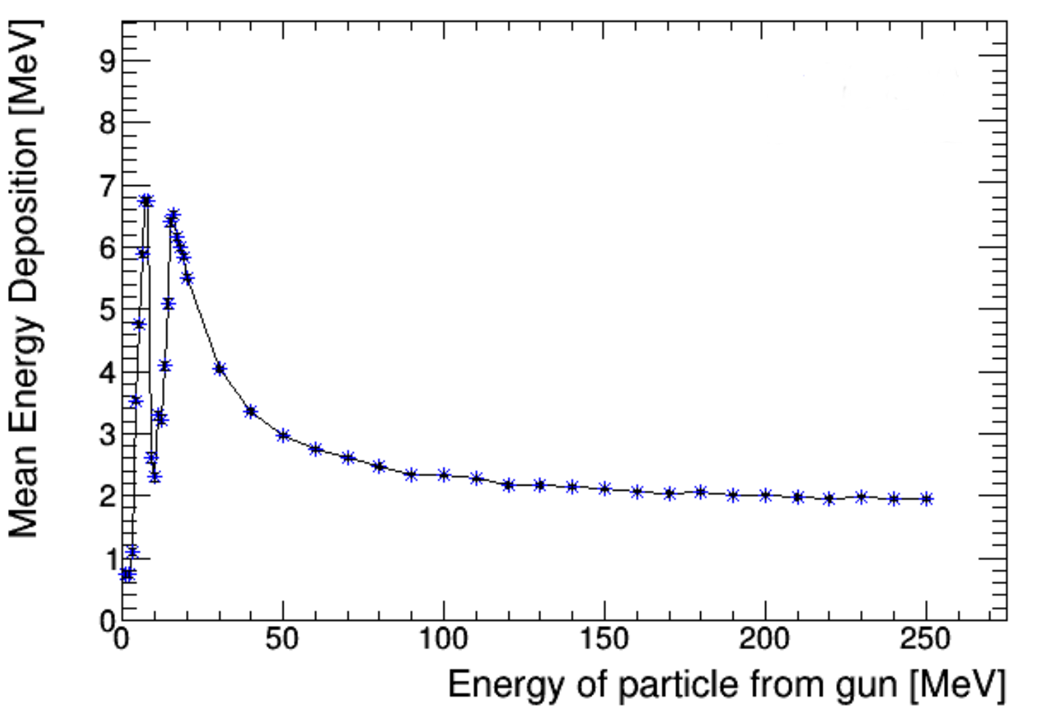
\includegraphics[width=\linewidth]{Chapter4/Figs/Raster/year1Plots/Muon_TiO2_med_eng.png}
  \captionof{figure}{$\mu$ mean energy deposition inactive component of the single bar, the sharp decrease in the energy deposited and varying deposition below 20\,MeV was due to the TiO$_2$ coating absorbing $\mu$ at lower energies.} 
  \label{fig:muon_0_250}
\end{minipage}%
\qquad
\begin{minipage}{.45\textwidth}
  \centering
  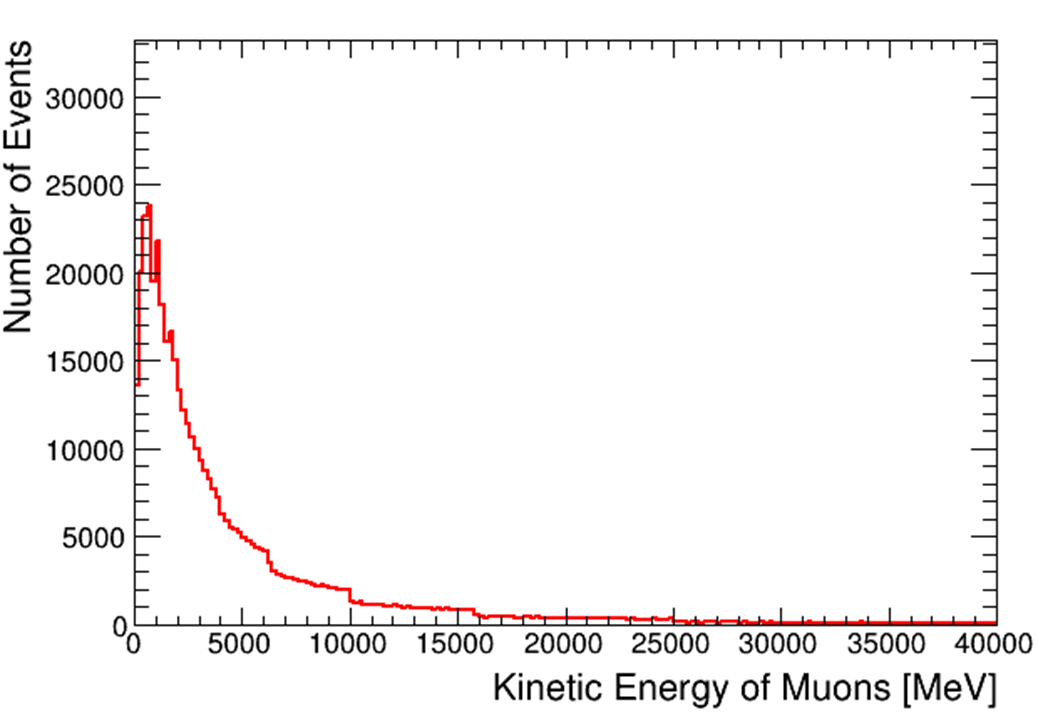
\includegraphics[width=\linewidth]{Chapter4/Figs/Raster/keMevCryMuons.png} 
  \captionof{figure}{Generated kinetic energy $\mu$ particles using the CRY library \cite{ieee_cry_2007} at sea level with latitude 53$^\circ$ (Liverpool's latitude) and date: 01 -- March -- 2021. 99\,\% + of generated $\mu$ particles are between 0.1\,GeV (100\,MeV) and 40\,GeV (40000\,MeV) kinetic energy.}
  \label{fig:keMevCryMuons}
\end{minipage}
\end{figure}

\begin{figure}[!h]
 \centering
 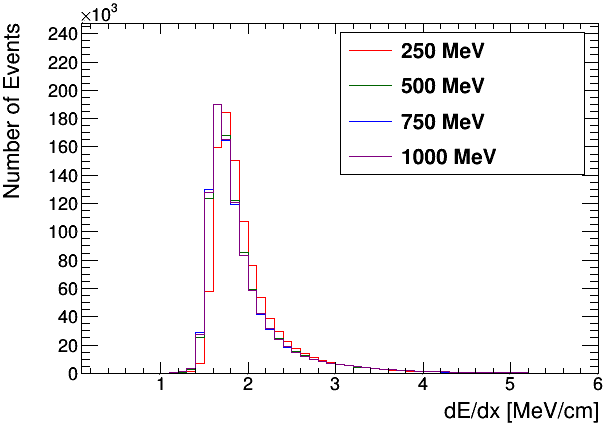
\includegraphics[width=0.7\linewidth]{Chapter4/Figs/Raster/year1Plots/muons_per_mev_cm.png}
 \captionof{figure}{dE/dx of $\mu$ through single plastic bar assuming a density of plastic of 1\,g\,cm$^{-3}$. Mearuemnts for plastic are similar to carbon. For carbon $\sim$ 2\,MeV\,cm$^{-1}$ is expected for dE/dx {\cite{Olive_2014}. Mean dE/dx for 250\,MeV, 500\,MeV, 750\,MeV, 1000\,MeV are respectively 1.9907 $\pm$  0.0005\,MeV\,cm$^{-1}$, 1.9387 $\pm$  0.0005\,MeV\,cm$^{-1}$, 1.9374 $\pm$  0.0005 MeV\,cm$^{-1}$, 1.9407 $\pm$  0.0005 MeV\,cm$^{-1}$.\\}}
 \label{fig:mev_per_cm_muons}
\end{figure}

As mentioned before the CRY library is very useful as it contains a large amount of relevant physics information with the latest version being 1.7 produced in 2012 \cite{hagmann2012cosmicCry}. The CRY library splits up the directions in the x,y and z by using cosine directions u (see equation\ref{equ:cos_u}), v (see equation \ref{equ:cos_v}) and w (see equation \ref{equ:cos_w}) respectively. However, whilst the generated cosine direction for u and v were very fine the binning for $\cos{w}$ was coarse. As a result, an 8-dimensional polynomial function was fitted to the $\cos{w}$ distribution in figure \ref{fig:Cry_GeneratedFit} to smooth out the distribution. The improvement to the distribution can be seen in figure \ref{fig:CrySmoothingCosTheta} where the finer binning of the cosine direction w in figure \ref{subFig:CrySmoothingCosine} leads to a smoother more accurate $\theta$ distribution in figure \ref{subFig:CrySmoothingTheta}. 

\begin{equation}
\alpha = \cos{u} = \frac{v_x}{\sqrt{v_x^2+v_y^2+v_z^2}}
\label{equ:cos_u}
\end{equation}

\begin{equation}
\beta = \cos{v} = \frac{v_y}{\sqrt{v_x^2+v_y^2+v_z^2}}
\label{equ:cos_v}
\end{equation}

\begin{equation}
\gamma = \cos{w} = \frac{v_z}{\sqrt{v_x^2+v_y^2+v_z^2}}
\label{equ:cos_w}
\end{equation}

\begin{figure}[!h]
 \centering
 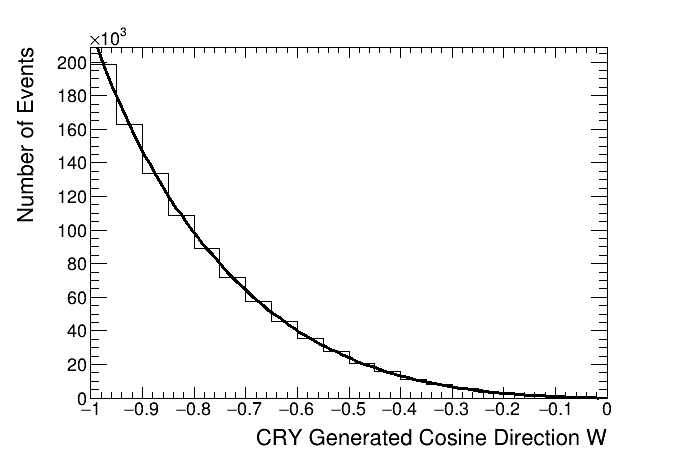
\includegraphics[width=0.7\linewidth]{Chapter4/Figs/CryFitCosW.png}
 \captionof{figure}{The generated angles for cosine direction W (z-axis) from the CRY library \cite{hagmann2007cosmic} for 1 million particles. Binning in CRY is 0.05 so an 8-dimensional polynomial was fitted to smooth the distribution.}
 \label{fig:Cry_GeneratedFit}
\end{figure}

\begin{figure}[!h]
\centering
\begin{subfigure}{.5\textwidth}
  \centering
  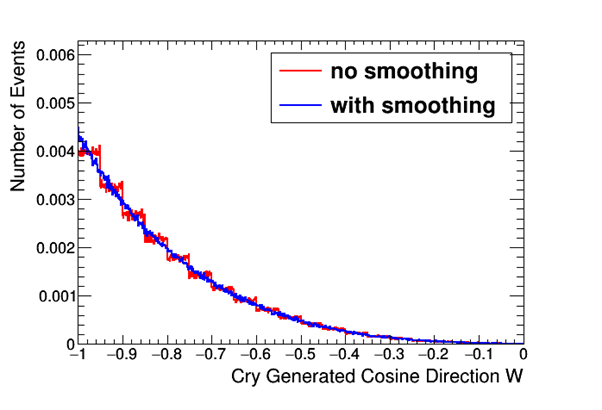
\includegraphics[width=\linewidth]{Chapter4/Figs/Raster/CryPlots/CrySmoothingCosine.png}
  \captionsetup{width=.9\linewidth}
  \caption{}
  \label{subFig:CrySmoothingCosine}
\end{subfigure}%
\begin{subfigure}{.5\textwidth}
  \centering
  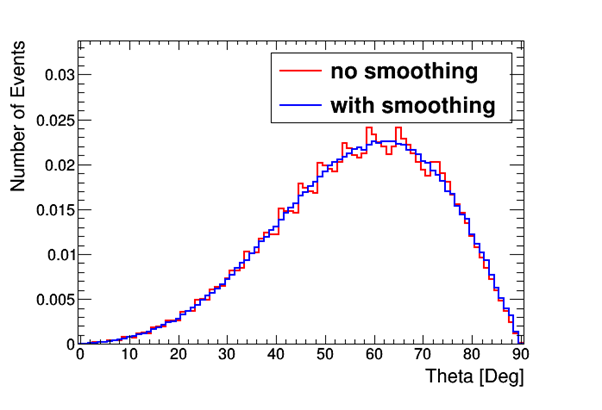
\includegraphics[width=\linewidth]{Chapter4/Figs/Raster/CryPlots/CrySmoothingTheta.png}
  \captionsetup{width=.9\linewidth}
  \caption{}
  \label{subFig:CrySmoothingTheta}
\end{subfigure}
\caption{How the smoothing affects the CRY distribution in $\cos{w}$ (see (a)) and $\theta$ (see (b)). The nonphysical peaks seen in the non-smoothed $\theta$ distribution are a direct result of CRY's coarse binning in $\theta$.}
\label{fig:CrySmoothingCosTheta}
\end{figure}

Now the $\theta$ distribution has been smoothed out accordingly the cosmic $\mu$ particles need to be back-projected. Back projection is where positions that CRY generates (see figure \ref{fig:cryxm_vs_cryym}) is taken as a ``target'' and then the $\phi$ values (a flat distribution between 0 -- 360$^\circ$) and smoothed $\theta$ values (see figure \ref{subFig:CrySmoothingTheta}) are used to project backwards to a point as a start vertex for a given radius. The larger the back projection radius the more accurate the simulation but the more computationally intensive it becomes. A back-projection of 100\,m is a reasonable approximation to simulate all incoming side on and top-down events. Figure \ref{fig:BackProjectionXY} shows how this looks in the x and y from a top-down perspective. The ``halo'' in figure \ref{fig:BackProjectionXY} is a result of the $\theta$ distribution seen in figure \ref{subFig:CrySmoothingTheta}. The rest of the simulated dome can be seen in figure \ref{fig:BackProjection_XZ_YZ} where the XZ and YZ distributions are very similar to each other. 


\begin{figure}[!h]
\centering
\begin{minipage}{.45\textwidth}
  \centering
  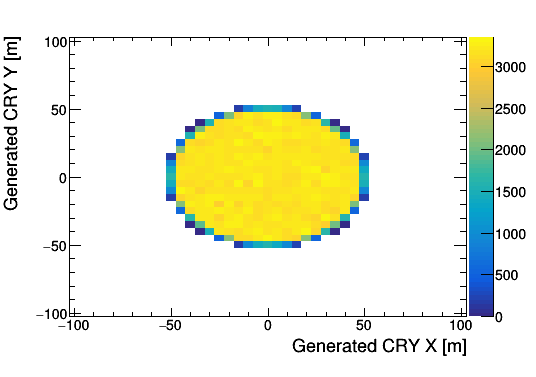
\includegraphics[width=\linewidth]{Chapter4/Figs/Raster/CryPlots/cryxm_vs_cryym.png}
  \captionof{figure}{Generated CRY X and Y positions in the simulation. A circle has been cut out of the generated square to give a flat $\phi$ distribution. All particles in CRY are generated at Z = 0.} 
  \label{fig:cryxm_vs_cryym}
\end{minipage}%
\qquad
\begin{minipage}{.45\textwidth}
  \centering
  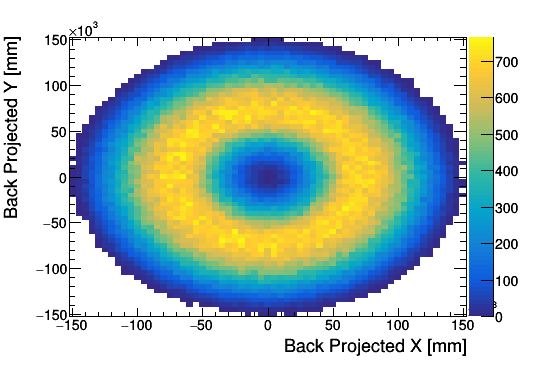
\includegraphics[width=\linewidth]{Chapter4/Figs/Raster/CryPlots/BackProjectionXY.png} 
  \captionof{figure}{Back projection of 100\,m in the (x,y) plane for the CRY library this represents the starting vertex for each particle generated in (x,y).}
  \label{fig:BackProjectionXY}
\end{minipage}
\end{figure}

\begin{figure}[!h]
\centering
\begin{subfigure}{.5\textwidth}
  \centering
  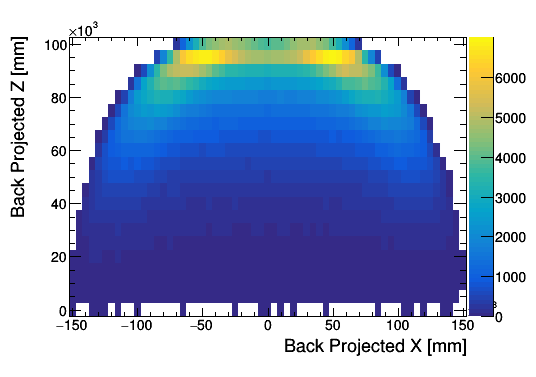
\includegraphics[width=\linewidth]{Chapter4/Figs/Raster/CryPlots/BackProjectionXZ.png}
  \captionsetup{width=.9\linewidth}
  \caption{}
  \label{subFig:BackProjectionXZ}
\end{subfigure}%
\begin{subfigure}{.5\textwidth}
  \centering
  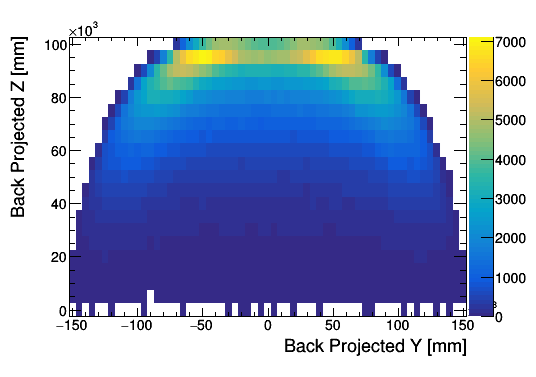
\includegraphics[width=\linewidth]{Chapter4/Figs/Raster/CryPlots/BackProjectionYZ.png}
  \captionsetup{width=.9\linewidth}
  \caption{}
  \label{subFig:BackProjectionYZ}
\end{subfigure}
\caption{Starting positions for the generated CRY distribution for (x,z) (see (a)) and (y,z) (see (b)) with a back projection of 100\,m.}
\label{fig:BackProjection_XZ_YZ}
\end{figure}

The impact of back-projection is relatively small when looking at where the particles cross the z Axis. As shown in figure \ref{fig:Crossed_atZ_XY_AndShort} when comparing a back projection of 1\,cm (figure \ref{subFig:CrossedZAxisShort}) to 100\,m (figure \ref{subFig:Crossed_atZ_XY}) both reproduce the circular distribution seen in figure \ref{fig:cryxm_vs_cryym} there is more scattering with more back-projection but this is a suitable trade-off for vastly more accurate tracks. 

\begin{figure}[!h]
\centering
\begin{subfigure}{.5\textwidth}
  \centering
  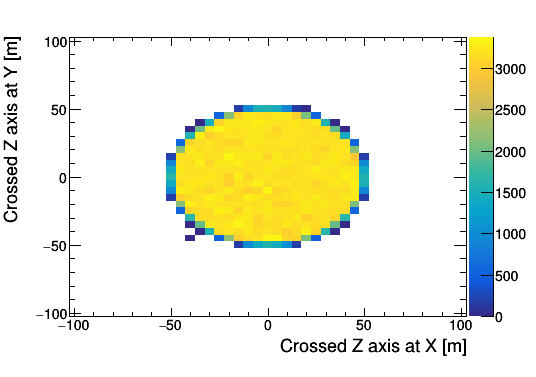
\includegraphics[width=\linewidth]{Chapter4/Figs/Raster/CryPlots/CrossedZAxisShort.png}
  \captionsetup{width=.9\linewidth}
  \caption{}
  \label{subFig:CrossedZAxisShort}
\end{subfigure}%
\begin{subfigure}{.5\textwidth}
  \centering
  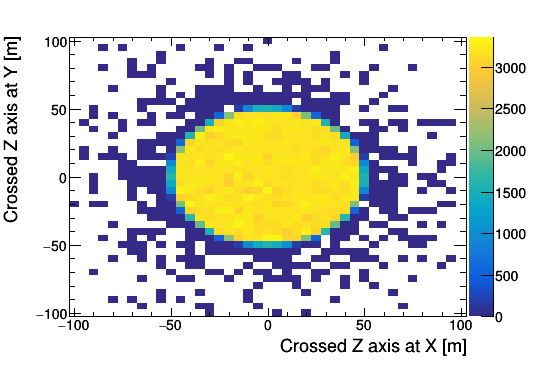
\includegraphics[width=\linewidth]{Chapter4/Figs/Raster/CryPlots/Crossed_atZ_XY.png}
  \captionsetup{width=.9\linewidth}
  \caption{}
  \label{subFig:Crossed_atZ_XY}
\end{subfigure}
\caption{How the generated CRY distribution crosses the Z-axis with only 1\,cm of back-projection (see (a)) vs 100\,m of back projection (see (b)). When the GEANT4 environment emulates the vacuum of space.}
\label{fig:Crossed_atZ_XY_AndShort}
\end{figure}

In addition, atmospheric effects need to be modelled. The atmosphere produces two main effects: it increases particle scattering (see figure \ref{fig:gen-scat_PhiTheta} and it increases the rate of secondaries produced (see figure \ref{fig:CRY_rates}). The CRY simulation takes the atmosphere into account \cite{hagmann2007monteCry} but only produces the particles that cross the Z axis at z = 0. As a result the secondaries produced by GEANT4 are also simulated by CRY thus resulting in some secondary particles being ``double simulated.'' This effect is most visible in figure \ref{fig:CRY_rates} where the rates in simulated air are overall $\sim$ 25\,\% higher than in G4$\textunderscore$Galactic (an environment in GEANT4 designed to emulate the vacuum of space). However, the paths of these particles are more accurate in the air and the secondaries produced inside a detector still need to be taken into account. For the most accurate cosmic modelling the air should be used whilst removing all secondaries that occur in the air i.e outside the detector. However, due to time constraints this was unable to be added to the simulation. 

\begin{figure}[!h]
\centering
\begin{subfigure}{.5\textwidth}
  \centering
  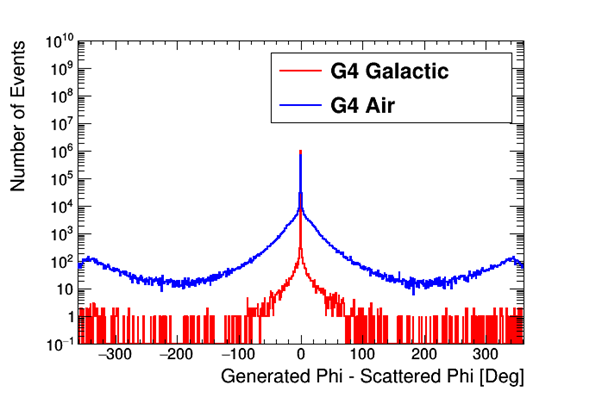
\includegraphics[width=\linewidth]{Chapter4/Figs/Raster/CryPlots/genPhi-scatPhi.png}
  \captionsetup{width=.9\linewidth}
  \caption{}
  \label{subFig:genPhi-scatPhi}
\end{subfigure}%
\begin{subfigure}{.5\textwidth}
  \centering
  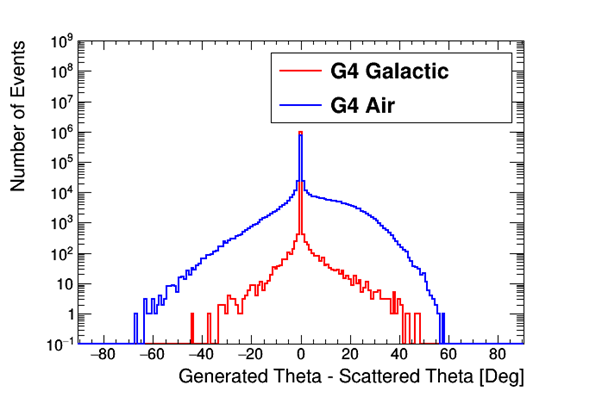
\includegraphics[width=\linewidth]{Chapter4/Figs/Raster/CryPlots/genTheta-scatTheta.png}
  \captionsetup{width=.9\linewidth}
  \caption{}
  \label{subFig:genTheta-scatPhi}
\end{subfigure}
\caption{How the Generated $\theta$ - scattered $\theta$ varies for air and galactic world material in GEANT4 (see (a)). And how the Generated $\phi$ - scattered $\phi$ varies for air and galactic world material in GEANT4 (see (b)).}
\label{fig:gen-scat_PhiTheta}
\end{figure}

\begin{figure}[!h]
 \centering
 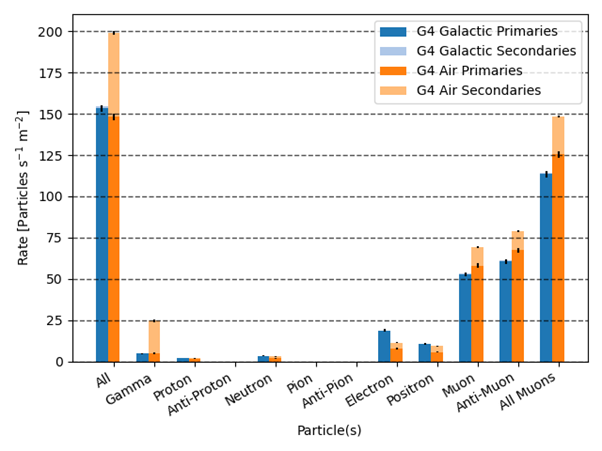
\includegraphics[width=0.7\linewidth]{Chapter4/Figs/Raster/CryPlots/CRY_rates.png}
 \captionof{figure}{How the rates vary depending on the world material in GEANT4. For Galactic world materials, secondary production is minimal. The rates are most accurate for Galactic world material but the paths will be more accurate for Air. Measured from a PVT block of 1\,m $\times$ 1\,m $\times$ 1\,cm to approximate particles s$^{-1}$ m$^{-2}$.} 
 \label{fig:CRY_rates}
\end{figure}

\clearpage
\section{Modelling TiO$_2$ Coating}
The plastic scintillating bars of the VIDARR detector are extruded at Fermilab and have been used in other experiments such as the T2K ND280 ECAL \cite{Allan_2013} Miner$\nu$a \cite{aliaga2014design} and in Mu2e as a cosmic ray veto \cite{Pla-Dalmau2014}. By simulating particles at the edge of a single bar as shown in figure \ref{fig:lengthAndSideViewBarMuon} the simulated dE/dx for a single bar can be measured by using the energy depoited in the bar and the length of each track in the bar for each particle. The impact that the TiO$_2$ coating has on the dE/dx depends on two variables, mass of particle and energy of the particle. When generating $\mu$ and protons between 0\,MeV -- 20\,MeV (figure \ref{fig:muonProton_TiO2}) the impact of both of these variables becomes clear. In figure \ref{fig:muonProton_TiO2} the TiO$_2$ coating is set to a thickness of 0.25\,mm which is the thickness Fermilab extrudes the coating \cite{Pla-Dalmau2014}.

\begin{figure}[!h]
\centering
\begin{subfigure}{.5\textwidth}
  \centering
  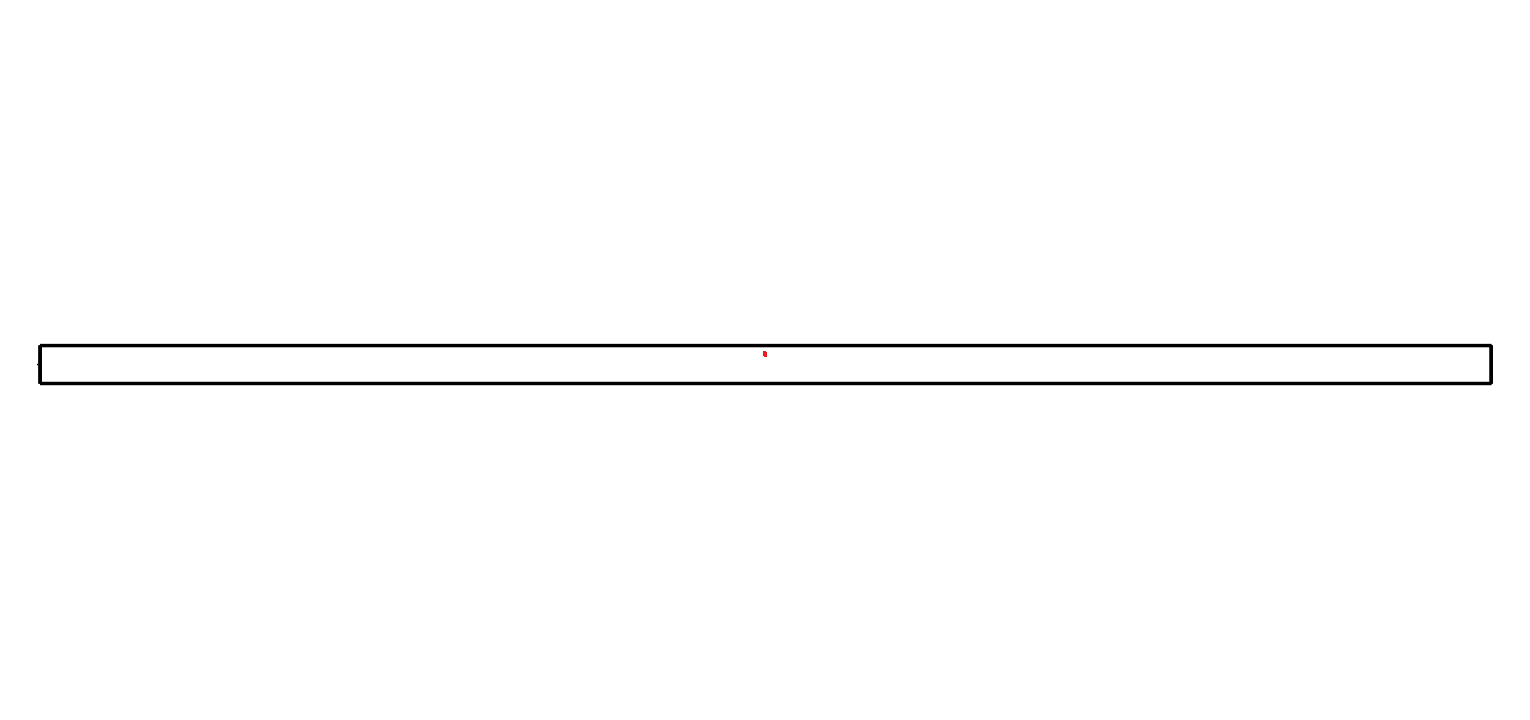
\includegraphics[width=\linewidth]{Chapter4/Figs/Raster/year1Plots/lengthOnViewBarMuon1530By720.png}
  \captionsetup{width=.9\linewidth}
  \caption{}
  \label{subFig:lengthOnViewBarMuon1530Square}
\end{subfigure}%
\begin{subfigure}{.5\textwidth}
  \centering
  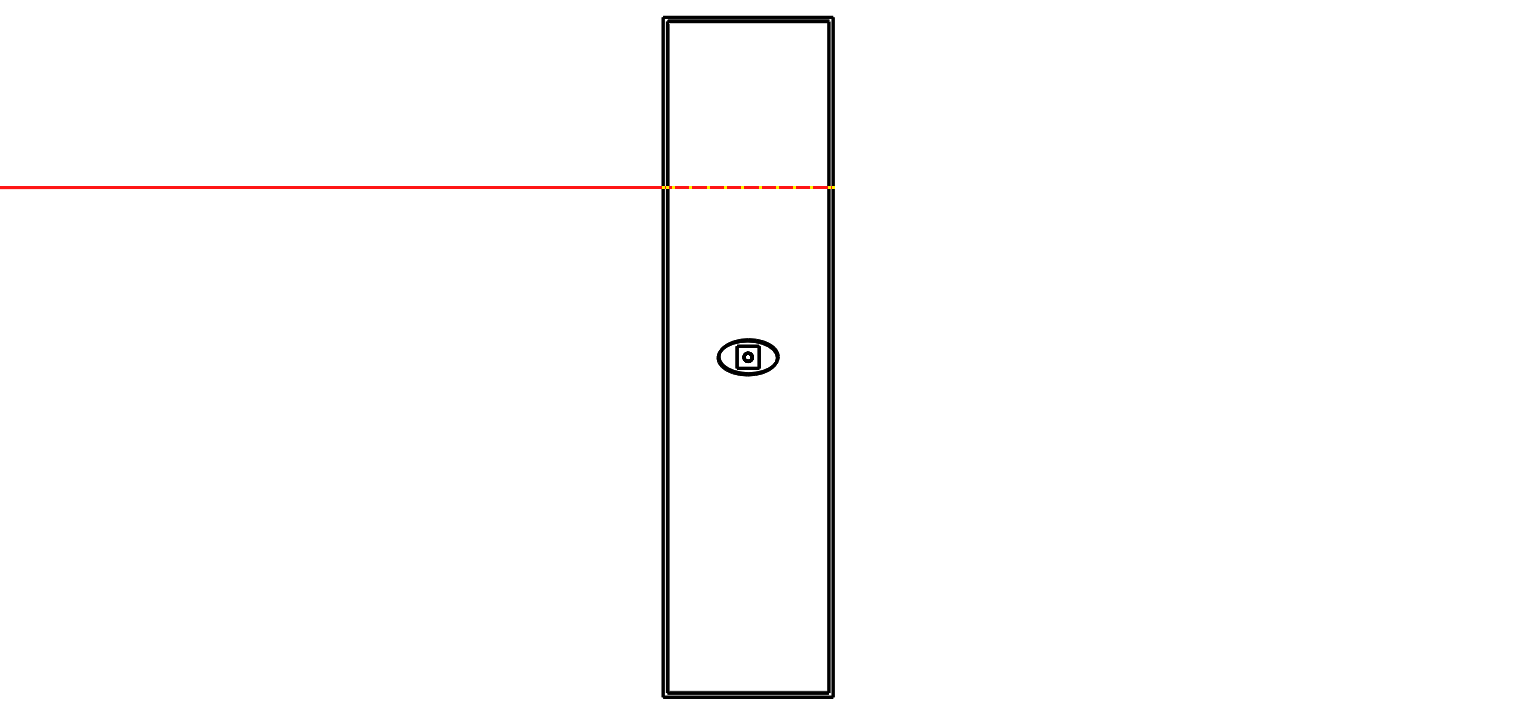
\includegraphics[width=\linewidth]{Chapter4/Figs/Raster/sideOnViewBarMuon1530By720.png}
  \captionsetup{width=.9\linewidth}
  \caption{}
  \label{subFig:sideOnViewBarMuon8}
\end{subfigure}
\caption{How a 20\,MeV $\mu$ particle penetrates through the coating and scintillator it is offset to ensure the effect from the TiO$_2$ coating is being correctly observed. The top down view (x,y) is shown in (a). The side on view (x,z) is shown in (b).}
\label{fig:lengthAndSideViewBarMuon}
\end{figure}


\begin{figure}[!h]
\centering
\begin{subfigure}{.5\textwidth}
  \centering
  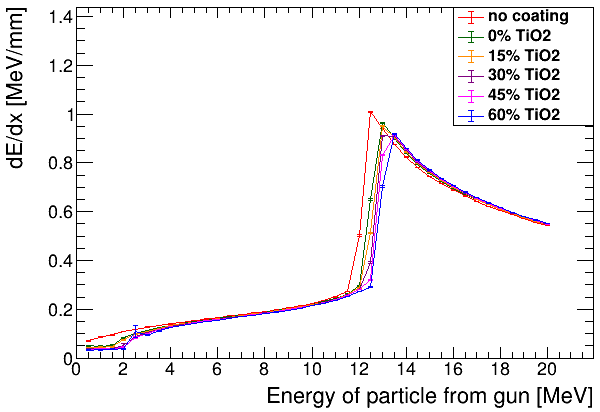
\includegraphics[width=\linewidth]{Chapter4/Figs/muon_TiO2_hybrid.png}
  \captionsetup{width=.9\linewidth}
  \caption{}
  \label{subFig:proton_TiO2}
\end{subfigure}%
\begin{subfigure}{.5\textwidth}
  \centering
  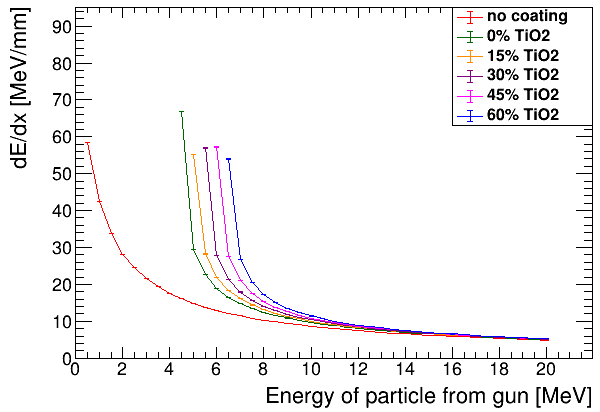
\includegraphics[width=\linewidth]{Chapter4/Figs/proton_TiO2_hybrid.png}
  \captionsetup{width=.9\linewidth}
  \caption{}
  \label{subFig:muon_TiO2}
\end{subfigure}
\caption{The average dE/dx for generated protons deposited in a single bar of scintillator the \%  of TiO$_2$ coating has significant impact except towards higher energies. The average dE/dx for generated cosmic $\mu$ deposited in a single bar of scintillator the \% of TiO$_2$ has some impact on the dE/dx at low energies.}
\label{fig:muonProton_TiO2}
\end{figure}

%The TiO$_2$ coating is 15\,\% TiO$_2$ to 85\,\% polythene \cite{aliaga2014design} \cite{Pla-Dalmau2014} with a thickness of 0.25\,mm \cite{Pla-Dalmau2014}. The correct amount of TiO$_2$ is now correctly implemented in the simulation for each of the 2660 bars in VIDARR. 

The percentage of TiO$_2$ to polythene is 15\,\% TiO$_2$:85\,\% polythene \cite{aliaga2014design} \cite{Pla-Dalmau2014} the simulated TiO$_2$ coating reflects this and is varied from 0\,\% -- 60\,\% in figure \ref{fig:muonProton_TiO2} to show the impact TiO$_2$ has on the $\mu$ and proton particles. The impact on $\mu$ dE/dx is only significant < 3\,MeV but the TiO$_2$ coating has a large impact on protons from 0\,MeV -- 12\,MeV. At low energies (0\,MeV -- 5\,MeV) protons don't penetrate very far and are unable to get through the 0.25\,mm coating regardless of composition. The percentage of TiO$_2$ also has an impact but it is less than than having a coating present at all. The dE/dx values are higher when the coating is present as the coating causes back scattering into the scintillating bar thus increasing energy deposition and dE/dx. This is important as it shows how unlikely it is for low energy protons and $\alpha$s are to penetrate the TiO$_2$ coating. In particular protons < 5\,MeV are unlikely to escape a single bar with a Ti0$_2$ of 15\,\%. As single bar events in the RMon and VIDARR detectors are often ignored it appears the TiO$_2$ coating will significantly reduce the number of proton and $\alpha$ events that will be considered as signal thus improving the signal to noise ratio. 

\section{Modelling Attenuation}\label{sec:GEANT4Simulation_ModellingAttenuation}
In order to characterise the physical effects of the detector, a test stand was set up by fellow collaborator George Holt. This test stand contained a single plastic scintillating bar where a $^{137}$Cs source was placed at 11 intervals across the bar from which attenuation of the 662\,keV peak could be measured. This is shown in figure \ref{fig:attenuationPlot} the exponential function (equation \ref{equ:attenuationFunction}) is used by the simulation to produce a data-driven model for the light attenuation in the simulation. The initial intensity is defined to be 13.1 $\pm$ 0.2\,PE by the Minuit2 fit with an attenuation length of 580 $\pm$ 60\,PE/cm and a $\chi^2$/NDF = 1.22. This should provide an accurate model for the attenuation within the bars of the VIDARR detector as it uses the same scintillator MPPC combination found in the VIDARR detector. At present no other experiments have this specific combination of scintillator shape, size and MPPC version so using these values should be more accurate than using values from the literature. 

\begin{equation}
P(x) = e^{-x/\lambda}
\label{equ:attenuationFunction}
\end{equation}

\begin{figure}[!h]
 \centering
 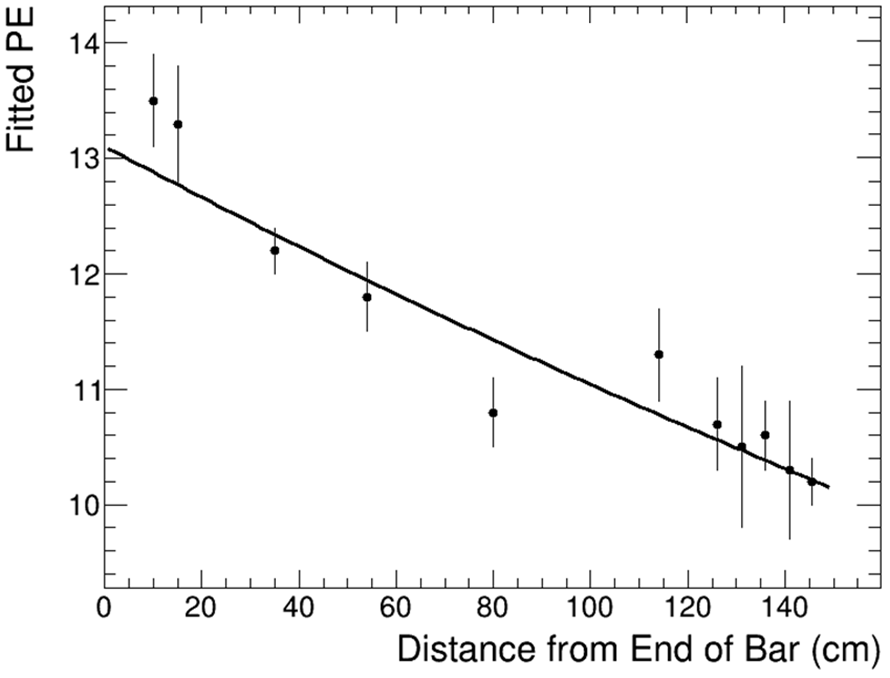
\includegraphics[width=0.7\linewidth]{Chapter4/attenuation_plot_no_box.png} 
 \captionof{figure}{The attenuation plot from the single bar test stand produced by George Holt. The attenuation length (amount of bar traversed to lose $\sim$ 63\,\%  of light, $\lambda$ in equation \ref{equ:attenuationFunction}) is 580 $\pm$ 60\,PE/cm. The initial intensity is 13.1 $\pm$ 0.2\,PE. $\chi^2$/NDF = 1.22.} 
 \label{fig:attenuationPlot}
\end{figure}

\section{Modelling Dark Noise}\label{sec:GEANT4Simulation_ModellingDarkNoise}
Another data-driven physical effect modelled in the simulation is the dark noise. Depending on temperature MPPCs will emit signals that are due to electronic effects rather than particle measurements. The dark noise was measured at room temperature over a 12 hour period by George Holt. The results in figure \ref{fig:pureDarkNoise} show Photo-electron (PE) peaks in units of mV with peaks for 1\,PE, 2\,PE and 3\,PE being clearly visible at 4.1\,mV, 8.2\,mV, and 12.3\,mV respectively. In order to measure the dark noise, an MPPC was put inside a container where no light would reach the sensor. 
\begin{figure}[!h]
 \centering
 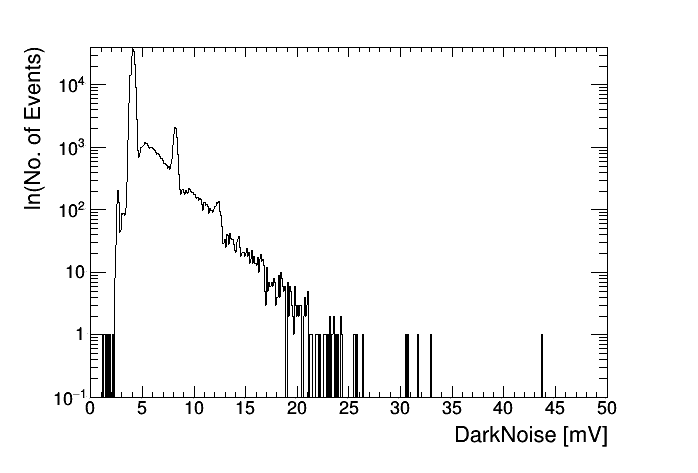
\includegraphics[width=0.7\linewidth]{pureDarkNoise_output.png}
 \captionof{figure}{Dark Noise from the MPPC taken over a period of $\sim$ 12\,hrs, taken by George Holt. The PE peaks for 1\,PE 2\,PE and 3\,PE can be seen at 4.1\,mv, 8.2\,mv and 12.3\,mv respectively. } 
 \label{fig:pureDarkNoise}
\end{figure}

The dark noise has two distinct components: the peaks, and the background surrounding the peaks. The background surrounding the peaks can be modelled using an exponential fit which is done in figure \ref{subFig:expFitOfDark}. In addition to the PE peaks and exponential noise there is also a pedestal peak (seen at 3\,mV in figure \ref{fig:pureDarkNoise}). This is the zero value for the MPPC and as such is discounted it's not relevant for measuring PE peaks which is what the analysis focuses on. The pedestal is useful for determining the gain and for calibration of channels but this is not the focus of the simulation which explicitly tries to emulate a believable signal post calibration. The removal of the pedestal peak and use of the aforementioned exponential fit is done in figure \ref{subFig:fittedDarkNoise}.
%The pedestal peak (seen at 3\,mV in figure \ref{fig:pureDarkNoise}) is also removed and an exponential is used past 13.7\,mV (see figure \ref{subFig:fittedDarkNoise}). 
\begin{figure}[!h]
\centering
\begin{subfigure}{.5\textwidth}
  \centering
  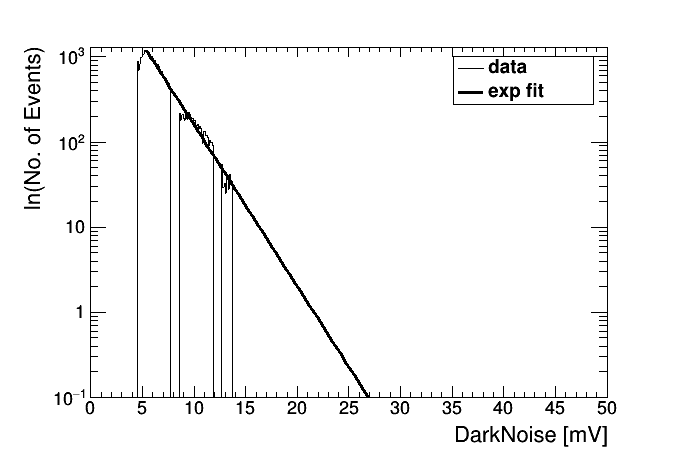
\includegraphics[width=\linewidth]{fit_of_dark_noise.png}
  \captionsetup{width=.9\linewidth}
  \caption{}
  \label{subFig:expFitOfDark}
\end{subfigure}%
\begin{subfigure}{.5\textwidth}
  \centering
  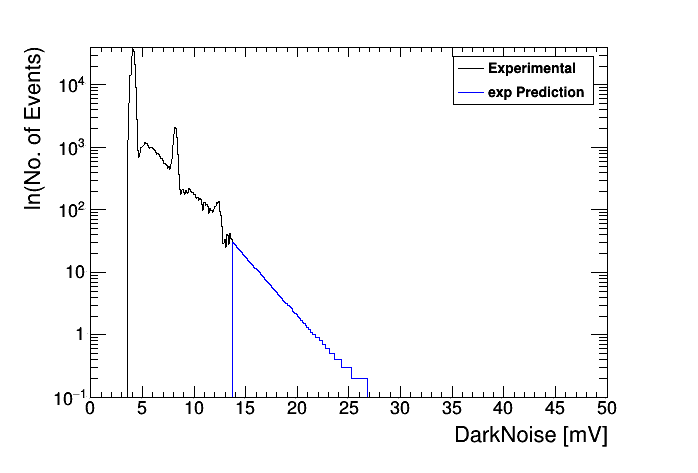
\includegraphics[width=\linewidth]{fittedDarkNoise_output.png}
  \captionsetup{width=.9\linewidth}
  \caption{}
  \label{subFig:fittedDarkNoise}
\end{subfigure}
\caption{Dark Noise from an MPPC taken over a period of $\sim$ 12\,hrs with an exponential fitted, with a $\chi ^2$ /DOF = 159.748 (see (a)). In (a) the fit of exponential function uses TFit to fit the after-pulsing of the MPPCs. The exponential fit is used past 13.7\,mV when the count rate drops below 10 and the conjoyed distribution can be seen in (b).}
\label{fig:fitting_of_non_peak_dark_noise}
\end{figure}

The results from figure \ref{fig:fitting_of_non_peak_dark_noise} can then be used to construct a cumulative probability distribution seen in figure \ref{fig:cumulative_prob_dark}. This probability distribution is what the simulation reads to reconstruct the dark noise distribution. During the simulation, a random dice is thrown and that probability is then converted back into a dark noise value which is then assigned to a random bar in the detector. Values past 13.7\,mV use the exponential fit. These events extrapolate directly from the exponential fit instead of reading from the probability distribution for more realistic results. The dark noise produced for a full detector over 10$^6$ events is shown in figure \ref{fig:individualDarkNoiseOld}. 

\begin{figure}[!h]
\centering
\begin{minipage}{.45\textwidth}
  \centering
  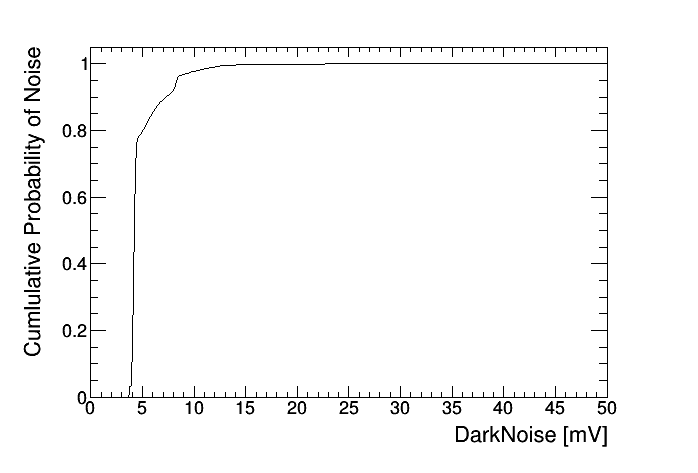
\includegraphics[width=\linewidth]{cumulative_prob_dark_noise.png}
  \captionof{figure}{Cumulative probability of the dark noise, which is converted to a table and then searched using the golden section search} 
  \label{fig:cumulative_prob_dark}
\end{minipage}%
\qquad
\begin{minipage}{.45\textwidth}
  \centering
  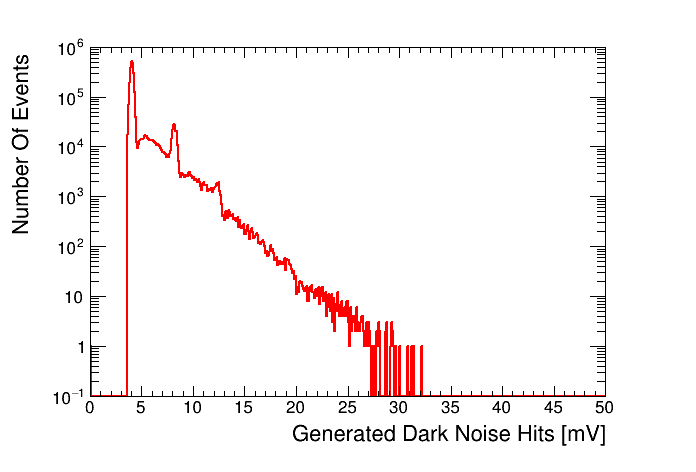
\includegraphics[width=\linewidth]{Chapter4/Figs/darkNoiseLog.png} 
  \captionof{figure}{The dark noise produced for the 2660 VIDARR detector with 10$^6$ events resulting in 3E6 dark noise hits. The exponential tail fit shown in \ref{fig:fitting_of_non_peak_dark_noise} has seamlessly connected to the rest of the distribution.}
  \label{fig:individualDarkNoiseOld}
\end{minipage}
\end{figure}

\section{Modelling Light Emission}\label{sec:GEANT4Simulation_ModellingLightEmission}
In order to measure light for a given amount of scintillating material, we need to consider several factors. For organic scintillators, the type of particle has a significant effect on the absolute light yield. The response of organic scintillators to charged particles can best be described by a relation between $dL/dx$ the fluorescent energy emitted per unit path length and $dE/dx$ the specific energy loss for the charged particle.  A widely used relation was first suggested by Birks \cite{birks_1964} is based on the assumption that a high ionisation density along the track of the particle leads to quenching from damaged molecules and a lowering of  scintillation efficiency. If we assume that the density of damaged molecules along the wake of the particle is directly proportional to the ionisation density we can represent their density by $B(dE/dx)$ where $B$ is a proportionality constant. Birks assumes that some fraction $k$ of these will lead to quenching\cite{knoll_2010}. A further assumption is that in absence of quenching the light yield is proportional to energy loss shown in equation \ref{equ:light_yield_proportional}. In equation \ref{equ:light_yield_proportional} $S$ is the normal scintillation efficiency \cite{birks_1964}. To account for the probability of quenching Birks then writes equation \ref{equ:Birks_formula}. Equation \ref{equ:Birks_formula} is commonly referred to as the Birks formula. The product $kB$ in equation \ref{equ:Birks_formula} is treated as an adjustable parameter to fit experimental data for a specific scintillator. Whereas $S$ in equation \ref{equ:Birks_formula} is particle specific and provides absolute normalisation \cite{knoll_2010}.  
\begin{equation}
\frac{dL}{dx} = S\frac{dE}{dx}
\label{equ:light_yield_proportional}
\end{equation}
\begin{equation}
\frac{dL}{dx} = \frac{S\frac{dE}{dx}}{1 + kB \frac{dE}{dx}}
\label{equ:Birks_formula}
\end{equation}
\\\\In this model molecules in the ionisation column are labelled ``damaged'' and ``undamaged'' for convenience, this nomenclature was coined by Birks and has been used since \cite{birks_1964}, \cite{craun_1970}, \cite{knoll_2010}. ``Damaged'' molecules are those which dissipate ionisation energy non-radiatively (quenching) and so lower the scintillation efficiency\cite{craun_1970} \cite{knoll_2010}. ``Damaged'' molecules occupy highly ionised or excited states, they de-excite quickly ($<$ 1 ns) to the ``undamaged'' condition \cite{craun_1970}. Some permanent damage will occur and does contribute to long term degradation of the scintillator but this is not relevant for quenching\cite{craun_1970}. B, therefore, is the ratio of ``damaged''/``undamaged'' molecules and k is the relative probability of quenching. kB is treated as a single adjustable parameter as there is no way to measure k or B separately \cite{craun_1970} \cite{knoll_2010}. kB is scintillator dependant only and will be referred to as a single entity: Birks' constant. For electrons above $\sim$ 125\,keV the response from the scintillator is linear \cite{craun_1970}. Birks' law (equation \ref{equ:Birks_formula}) also becomes linear for fast electrons \cite{knoll_2010}. As a result, quenching may not be sufficient for modelling fast electrons as will be expanded upon in section \ref{sec:GEANT4Simulation_quenchingLoss}. 
\section{MINER$\nu$A Birks' Constant}\label{sec:GEANT4Simulation_MINERvABirksConstant}
In equation \ref{equ:Birks_formula} the parameters $kB$ and $S$ are empirically determined. $S$ is a normalisation parameter that is particle dependent and kB is the Birks' constant for the scintillator and is particle independent. The MINER$\nu$A collaboration \cite{aliaga_2015} also uses the same scintillator as the VIDARR detector \cite{aliaga_2014}, the collaboration determined the value of the of kB to be 0.0905 $\pm$ 0.015\,mm/MeV at best fit. This Birks parameter was obtained by using GEANT4 MC data, which is the same approach by which VIDARR has obtained its birks parameter (kB = 0.0947 $\pm$ 0.00001).Both the VIDARR and MINER$\nu$A approach use the GEANT4 Bertini cascade model when attempting to measure the Birks' constant $kB$ \cite{Heikkinen_2003}. 
\\\\GEANT4 uses approximations of physics called physics lists. Each physics list has ranges and models that make them suitable under different circumstances. For VIDARR/RMon when simulating the full detector the shielding physics list is used for it's more accurate neutron modelling. However, for modelling and approximating GEANT4's light output the standard Quark Gluon String physics list (QGSP) was used. This was done as the MINER$\nu$a collaboration ahd used this list and it ave good results for light output \cite{Patrick_2018}. The steps have to remain course in GEANT4 otherwise the $kB$ parameter changes  \cite{aliaga_2015}. This is why the EMY physics lists were not used, even though they simulate smaller steps and so would potentially simulate stopping better. Then energy range for the MINER$\nu$A signal is of order $\sim$ 1\,GeV, whereas the energy range for VIDARR's signal is $\sim$ 0\,MeV -- 10\,MeV. However, a major source of noise for VIDARR is cosmic $\mu$ which have energies $\sim$ 1\,GeV and protons with energies between 0-10\,MeV as a result of fast neutrons. Using the MINER$\nu$A data requires going to higher energies (lower $dE/dx$) in order to ensure similar results in the $dL/dx$ fit.  
\\\\The results of the MINER$\nu$A Birks' law investigation concluded that a Birks' constant of 0.0905 $\pm$ 0.015\,mm/MeV was the most accurate value for the scintillator \cite{aliaga_2015}. Whilst the MINER$\nu$A experiment measures protons with an energy range of 0\,MeV-500\,MeV and the particles of VIDARR's interest are $\overline{\nu_{e}}$s with energy range between 0\,MeV-10\,MeV the Birks' constant is the same regardless. This is because Birks' law is a representation of the scintillator itself and therefore is not particle or energy-dependent. The amount of saturation in the scintillator that Birks' constant represents is constant in all cases. The kB value used in the simulation is the MINER$\nu$A value, but ultimately it makes a minimal difference as the values obtained by VIDARR and MINER$\nu$A are so similar. 
\section{Approximating GEANT4's Light Output}\label{sec:GEANT4Simulation_MonteCarloBirksLaw}
Modelling photons in GEANT4 is computationally expensive it requires simulating optical photon tracks at every energy deposition for a given amount of energy. A scintillation yield of $10^5$\,photons/MeV is considered a good approximation for a plastic scintillator as it covers the energy range of interest (0\,MeV -- 10\,MeV) and significantly above \cite{craun_1970}. But with such a high scintillation yield the slowdown observed in this simulation especially at higher energies is extreme. This slowdown can be somewhat alleviated by counting the number of photons and then killing the optical photon tracks. As the number of photons determines the quenching, but even the ``count and kill'' method is computationally expensive. So whilst the count and kill method was used for determining Birks' law, once the light was characterised this method was abandoned due to its high computational load.
\\\\In order to accurately model the light output two new simulations of the scintillator were required to quantify the effects of the Birks' constant ($kB$ in the equation \ref{equ:Birks_formula}). Both of them required the removal of all wavelength shifting fibres and MPPCs, they are just scintillators. The first model is a ``slice model'' that is 1\,mm thick and had a cross-section of 0.2\,m by 0.2\,m (see figure \ref{fig:lengthAndSideViewSliceElectron780Square}). This model allows for the approximations $dL/dx \approx \Delta L / \Delta x$ and $dE/dx \approx \Delta E / \Delta x$ to be used. The second model was a ``slab'' model (figure \ref{fig:electrons_viewed_in_slab}) that was 2\,m thick and had a cross-section of 0.2\,m by 0.2\,m. This model is used for determining quantifying light production from Birks' approximation and comparing that light output to the simulated GEANT4 values. Both models had particle energy ranges of 0\,MeV-100\,MeV.

\begin{figure}[!h]
\centering
\begin{subfigure}{.5\textwidth}
  \centering
  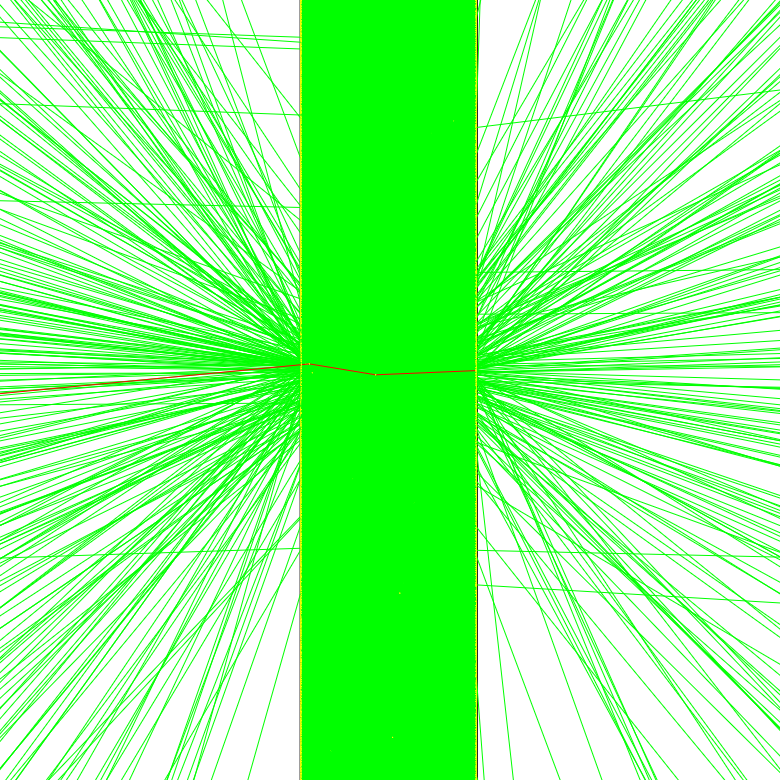
\includegraphics[width=0.7\linewidth]{Chapter4/Figs/Raster/lengthOnViewSliceElectron780Square.png}
  \captionsetup{width=.9\linewidth}
  \caption{}
  \label{subFig:lengthOnViewSliceElectron780Square}
\end{subfigure}%
\begin{subfigure}{.5\textwidth}
  \centering
  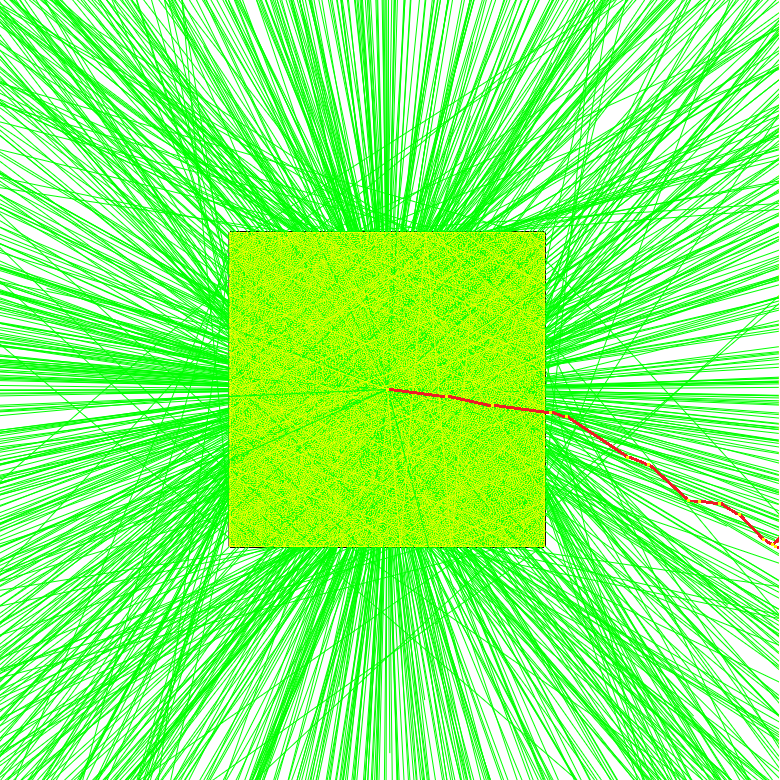
\includegraphics[width=0.7\linewidth]{Chapter4/Figs/Raster/sideOnViewSliceElectron780Square.png}
  \captionsetup{width=.9\linewidth}
  \caption{}
  \label{subFig:sideOnViewSliceElectron780Square}
\end{subfigure}
\caption{A 1\,MeV e$^-$ particle (the red track) being simulated in a slice of plastic scintillator measuring 0.2\,m by 0.2\,m in (y,z) with 1\,mm thickness in x. Optical photons (the green tracks) are simulated to show how many are produced even over such a short distance at relatively low energies. (a) shows the side on view (x,z). (b) shows the length on view (y,z)}
\label{fig:lengthAndSideViewSliceElectron780Square}
\end{figure}

The ``slice'' model was used to determine the $S$ values for every particle in equation \ref{equ:Birks_formula}, once those had been obtained the $kB$ value of 0.0905 $\pm$ 0.015\,mm/MeV obtained from MINER$\nu$A was also used \cite{aliaga_2015}. By using the approximations $dL/dx \approx \Delta L / \Delta x$ and $dE/dx \approx \Delta E / \Delta x$ and using $\Delta L = L_{\textrm{end}} - L_{\textrm{start}} $ where in the simulation it is known that the light at the start of the step $L_{\textrm{start}} = 0$ and $L_{\textrm{end}}$ is the light at the end of each GEANT4 equation \ref{equ:light_produced} can be inferred. Using equation \ref{equ:light_produced} the light yield can now be calculated for the following particles were: $e^-$,$e^+$,$p$,$\bar{p}$,$\pi^+$,$\pi^-$,$\mu^-$,$\mu^+$,$\alpha$,$\bar{\alpha}$.

\begin{figure}[!h]
\centering
\begin{subfigure}{.5\textwidth}
  \centering
  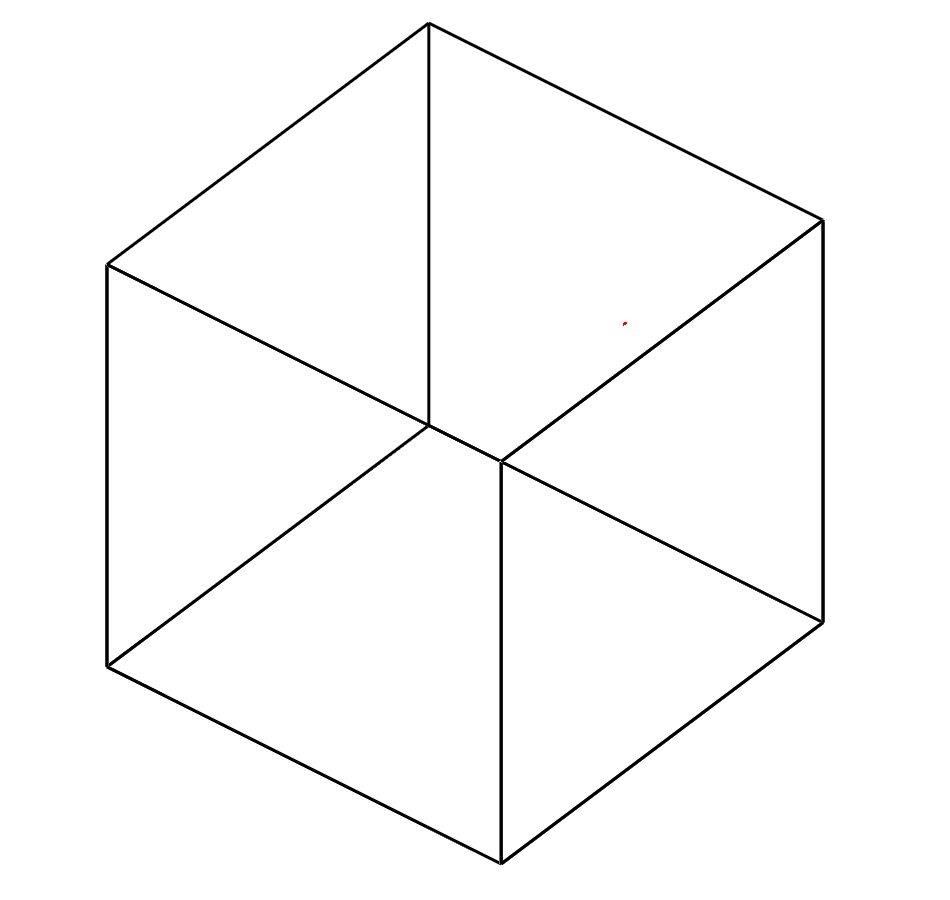
\includegraphics[width=0.7\linewidth]{Chapter4/Figs/newSlab3d950By900Red.png}
  \captionsetup{width=.9\linewidth}
  \caption{}
  \label{subFig:electronsSlab3d}
\end{subfigure}%
\begin{subfigure}{.5\textwidth}
  \centering
  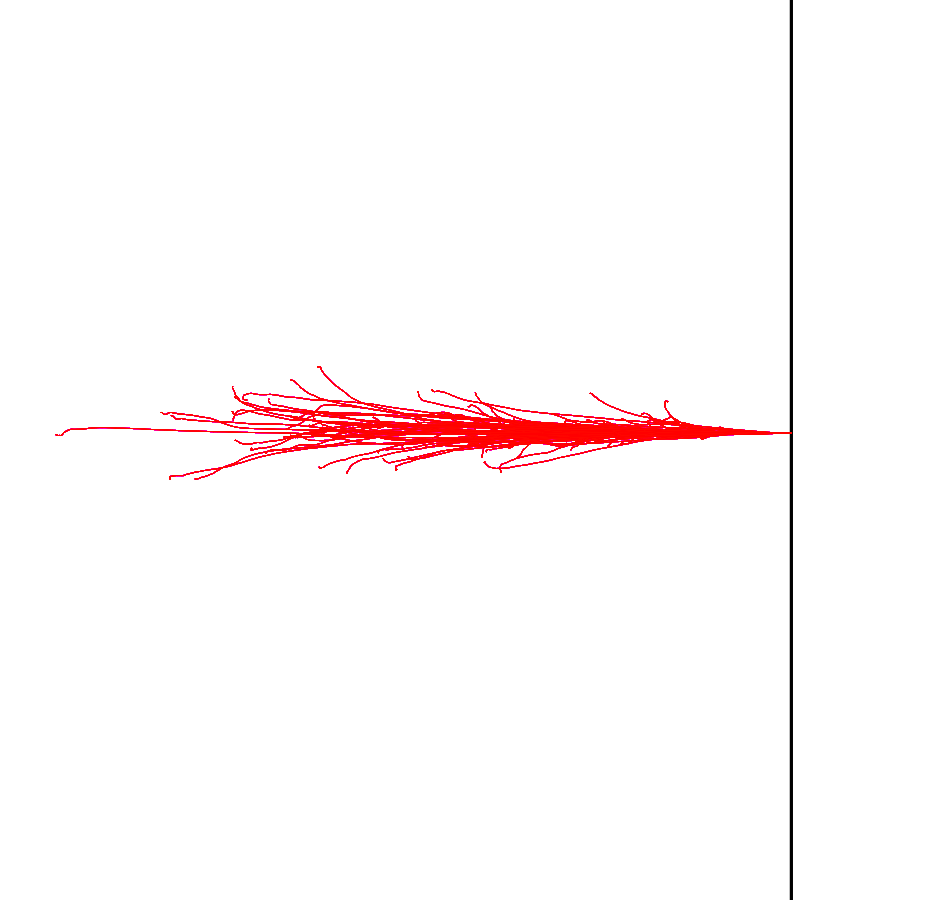
\includegraphics[width=0.7\linewidth]{Chapter4/Figs/newSlabSideOnView950By900Red.png}
  \captionsetup{width=.9\linewidth}
  \caption{}
  \label{subFig:electronsSlabSideOn}
\end{subfigure}
\caption{One hundred e$^-$s in a large slab of scintillator with a generated kinetic energy from 0\,MeV -- 100\,MeV. The slab of scintillator is 200\,m $\times$ 200\,m $\times$ 200\,m. Figure \ref{subFig:electronsSlab3d} shows the 3D view of the slab and figure \ref{subFig:electronsSlabSideOn} shows the zoomed in side on view of the e$^-$s travelling down the x direction.}
\label{fig:electrons_viewed_in_slab}
\end{figure}

\begin{equation}
L_{\textrm{end}}\approx \Delta x \left(\frac{S\frac{\Delta E}{\Delta x}}{1 + kB \frac{\Delta E}{\Delta x}}\right) 
\label{equ:light_produced}
\end{equation}
\\The approximations that Birks' law predicts for $p$,$\overline{p}$,$\pi^+$,$\pi^-$,$\mu^-$,$\mu^+$,$\alpha$,$\overline{\alpha}$ are very close to the model of light that GEANT4 predicts. The deviation from GEANT4 is at the worst at 100\,MeV where there is a deviation of $\sim$ $3\%$ in light output between GEANT4 and the Birks approximation of protons and anti-protons seen in figure \ref{fig:proton_aproton_light} (\ref{subFig:proton_light} represents protons and \ref{subFig:aproton_light} represents anti-protons). In figure \ref{fig:proton_aproton_light} the Brik's approximation is a closer fit to the data than the simulated light fit which is a square function ($L = aE^2 + bE+ c$). A full table of S values can be seen in table \ref{tab:sValueTable}. Note how the positron S value is above the maximum photon limit of 10$^5$. 

\begin{table*}[!h]
\centering
\begin{tabular}{lllll}  
\toprule
Particle       & kB [mm/MeV]        & S [photons/MeV]   & Fitting Range [MeV/mm] & $\chi^2$/NDF\\
\midrule
$\alpha$       & 0.0905 $\pm$ 0.015 & 9963.5  $\pm$ 0.3 & 0 -- 200               & 98.3163 \\
$\bar{\alpha}$ & ....               & 9973.1  $\pm$ 0.2 & 0 -- 200               & 85.7297 \\
$P$            & ....               & 9967.5  $\pm$ 0.3 & 0 -- 200               & 297.246 \\
$\bar{P}$      & ....               & 9987.1  $\pm$ 0.3 & 0 -- 200               & 607.475 \\
$\pi^+$        & ....               & 9978.2  $\pm$ 0.3 & 0 -- 200               & 9762.33 \\
$\pi^-$        & ....               & 9985.3  $\pm$ 0.3 & 0 -- 200               & 13193.4 \\
$\mu^-$        & ....               & 10043.1 $\pm$ 0.3 & 0 -- 200               & 42026.8 \\
$\mu^+$        & ....               & 10027.2 $\pm$ 0.3 & 0 -- 200               & 23874.9 \\
$e^-$          & ....               & 9418    $\pm$ 2   & 2 -- 19                & 13.4511 \\
$e^+$          & ....               & 9276    $\pm$ 2   & 2 -- 19                & 26.3355 \\
\bottomrule  
\end{tabular}
\caption{The kB and S values for each particle in the simulation were found via Birks' equation. The kB value is from MINER$\nu$A and is the same for each particle. The $\chi^2$/NDF values are high due to the high number of statistics and large fluctuation in each distribution (see appendix  \ref{appendixD:dldxVsDedxPlots} for a full list of plots). This isn't concerning so long as the simulated light from GEANT4 roughly matches the Birks' approximation.}
\label{tab:sValueTable}
\end{table*}

\begin{figure}[!h]
\centering
\begin{subfigure}{.5\textwidth}
  \centering
  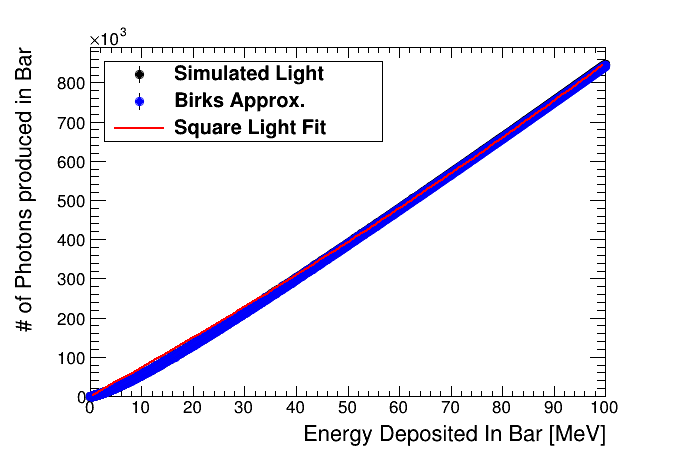
\includegraphics[width=\linewidth]{Chapter4/Figs/protonBirksSlab_simAndApproxLight.png}
  \captionsetup{width=.9\linewidth}
  \caption{}
  \label{subFig:proton_light}
\end{subfigure}%
\begin{subfigure}{.5\textwidth}
  \centering
  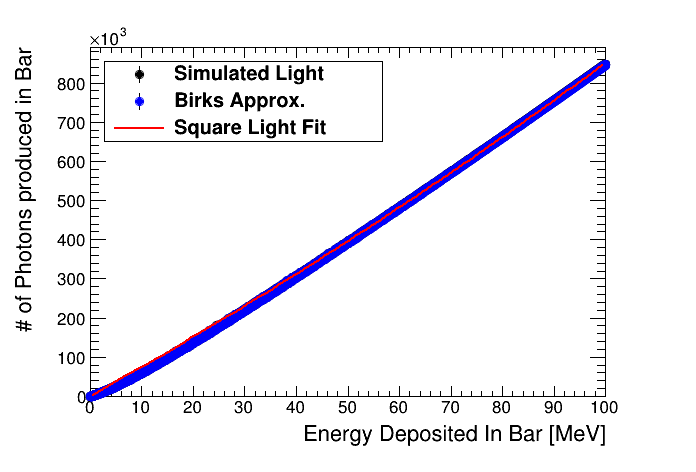
\includegraphics[width=\linewidth]{Chapter4/Figs/aProtonBirksSlab_simAndApproxLight.png}
  \captionsetup{width=.9\linewidth}
  \caption{}
  \label{subFig:aproton_light}
\end{subfigure}
\caption{Proton and anti-proton light output compared to the birks approximation and a square fit to the light output in GEANT4.}
\label{fig:proton_aproton_light}
\end{figure}

However, the light yield for e$^-$ and e$^+$ (see figure \ref{fig:electron_positron_light}) varies more significantly. At 100\,MeV a variation of $\sim$ 15\,\% is seen in both the e$^-$ (figure \ref{subFig:electron_light}) and e$^+$ (figure \ref{subFig:positron_light}). The reason for this discrepancy are the low values of $dE/dx$ for e$^-$ and e$^+$. Whilst the Birks' law fits well between 1\,MeV/mm -- 19\,MeV/mm the higher energy values for e- and e+ tend to have lower values of $dE/dx$ which the Birks' law does not fit well. The solution is to fit a 2d Square polynomial for $dE/dx$ vs. $dL/dx$ between 0\,MeV/mm -- 2\,MeV/mm (coefficients and $\chi^2$/NDFs are seen in table \ref{tab:e-e+SquareDlDeTable}). This additional correction is used in figure \ref{fig:square_electron_positron_light} for both e$^-$ (figure \ref{subFig:square_electron_light}) and e$^+$ (figure \ref{subFig:square_positron_light}) and results in a much more accurate approximation of GEANT4's light yield. The reason for large discrepancy is due to range straggling as higher energy e$^-$ and e$^+$ particles travel much further than the other charged particles simulated and as such deposit much lower values of $dE/dx$ as they travel on average \cite{knoll_2010}. This range straggling is insignificant for the other particles simulated for example for protons or alphas the straggling amounts to a few percent of the mean range \cite{knoll_2010}. 
% However, the light yield for electrons and positrons seen in figure \ref{fig:electron_positron_light} varies more significantly. At 100\,MeV a variation of $\sim$ 15\,\% is seen in the electrons (figure \ref{subFig:electron_light}) and a variation and a variation of $\sim$ 20\,\% is seen in positrons (figure \ref{subFig:positron_light}). In figure \ref{fig:electron_positron_light} the simulated light which is a square function more accurately represents the GEANT4 light predictions. Figure \ref{fig:square_electron_positron_light} shows this approximation inputted instead. There is a slight variation between the simulated light fit and the square approximation seen in figures \ref{subFig:square_electron_light} (e$^-$) and \ref{subFig:square_positron_light} (e$^+$). This is because the simulated light fit fits the whole light distribution whereas the light produced by the approximation in simulation is produced per GEANT4 step. Despite this, the square approximation for e$^-$ light ($L = 0.9347E^2 + 10340E - 0.1000$) had a variation of 0.7\,\% at 100\,MeV and the square approximation of the e$^+$ light ($L = 0.9716E^2 + 10350E -0.1000$) had a variation of 0.3\,\% at 100\,MeV. 
\begin{figure}[!h]
\centering
\begin{subfigure}{.5\textwidth}
  \centering
  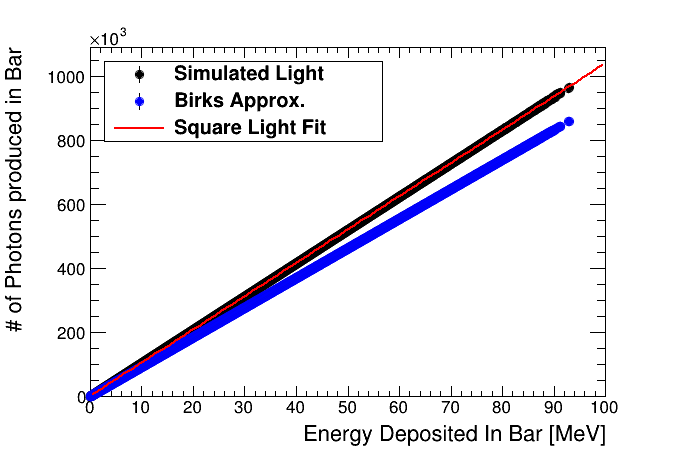
\includegraphics[width=\linewidth]{Chapter4/Figs/e-BirksSlab_simAndApproxLight.png}
  \captionsetup{width=.9\linewidth}
  \caption{}
  \label{subFig:electron_light}
\end{subfigure}%
\begin{subfigure}{.5\textwidth}
  \centering
  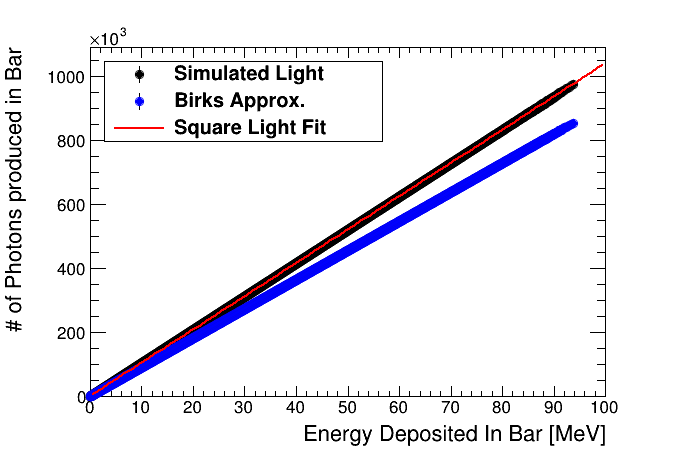
\includegraphics[width=\linewidth]{Chapter4/Figs/e+BirksSlab_simAndApproxLight.png}
  \captionsetup{width=.9\linewidth}
  \caption{}
  \label{subFig:positron_light}
\end{subfigure}
\caption{Electron, Positron light output compared to the birks approximation and a square fit to the light output in GEANT4}
\label{fig:electron_positron_light}
\end{figure}

\begin{table*}[!h]
\centering
\begin{tabular}{lllll}  
\toprule
Particle       & a                 & b                 & c                 & $\chi^2$/NDF\\
\midrule
$e^-$          & -553.3 $\pm$ 0.7  & 9220.5 $\pm$ 0.5  & 258.10 $\pm$ 0.07 & 39.9469 \\
$e^+$          & -651.1 $\pm$ 0.8  & 9266.5 $\pm$ 0.5  & 251.59 $\pm$ 0.08 & 31.0016 \\
\bottomrule  
\end{tabular}
\caption{The e$^-$ and e$^+$ $dE/dx$ vs $dL/dx$ for 0\,MeV/mm -- 2\,MeV/mm. The equation is in the form $dL/dx = a (dE/dx) + b dE/dx + c$. The fit for both have high $\chi^2$/NDF which is not a concern as it improves the light approximation significantly and is partially a result of high statistics. }
\label{tab:e-e+SquareDlDeTable}
\end{table*}

\begin{figure}[!h]
\centering
\begin{subfigure}{.5\textwidth}
  \centering
  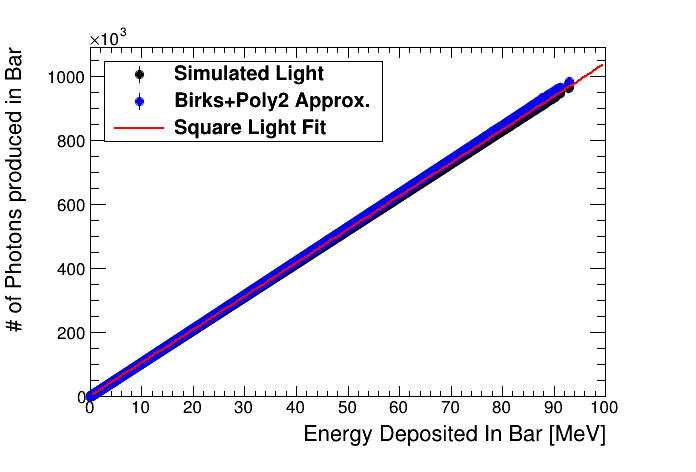
\includegraphics[width=\linewidth]{Chapter4/Figs/e-Birks-Poly2Slab_simAndApproxLight.png}
  \captionsetup{width=.9\linewidth}
  \caption{}
  \label{subFig:square_electron_light}
\end{subfigure}%
\begin{subfigure}{.5\textwidth}
  \centering
  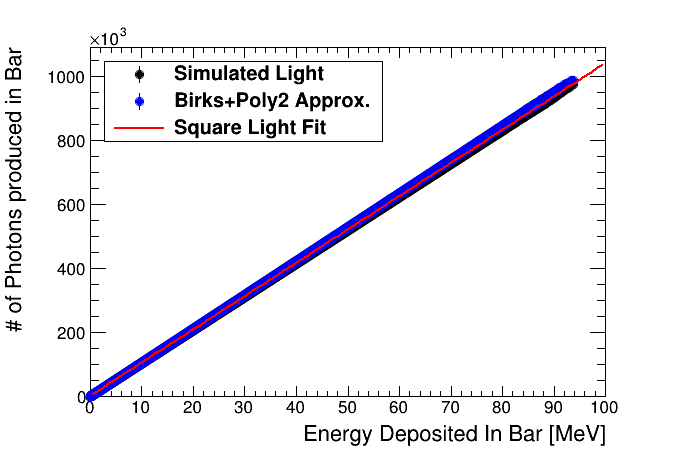
\includegraphics[width=\linewidth]{Chapter4/Figs/e+Birks-Poly2Slab_simAndApproxLight.png}
  \captionsetup{width=.9\linewidth}
  \caption{}
  \label{subFig:square_positron_light}
\end{subfigure}
\caption{Electron and positron light output from simulation compared to a GEANT4 step square approximation}
\label{fig:square_electron_positron_light}
\end{figure}

In order to convert between light and energy the scintillator's response to e$^-$ needs to be considered. The light of an e$^-$ is the highest amount of light per MeV that a particle can deposit. This MeV electron equivalent (MeVee) is a special nomenclature used to describe the absolute light yield. The square light fit $L = aE^2 + bE +c$ seen in figures \ref{subFig:electron_light} and \ref{subFig:square_electron_light} can then be used to convert between light and energy. Equation \ref{equ:MeV_electron_equivalent_square} shows the values for the $L^2$ fit in \ref{subFig:electron_light} and \ref{subFig:square_electron_light}. The $E^2$ coefficient is << than the coefficient for E and as a result the fit was change to a linear fit, the values for which are shown in equation \ref{equ:MeV_electron_equivalent_linear} this fit as a $\chi^2$/NDF of 9.01531. Equation \ref{equ:MeV_electron_equivalent_linear} is then differentiated to obtain $dL/dE$ in equation \ref{equ:MeV_electron_equivalent_dl/de}. Equation \ref{equ:MeV_electron_equivalent_dl/de} is then rearranged so that light output can be converted into energy in equation \ref{equ:MevLightConversion}. As mentioned earlier the approximation made is that $\Delta E \sim dE$ and $\Delta L \sim dL$. Where the $\sim$ $\Delta L$ is the light produced in the GEANT4 step and $\sim$ $\Delta E$ is the energy produced in the step according to that light output.
\begin{equation}
L = 0.0876519E^2 + 10396.7E - 263.7
\label{equ:MeV_electron_equivalent_square}
\end{equation}
\begin{equation}
L = 10401.2 - 281.307
\label{equ:MeV_electron_equivalent_linear}
\end{equation}
\begin{equation}
\frac{dL}{dE} = 10401.2
\label{equ:MeV_electron_equivalent_dl/de}
\end{equation}
\begin{equation}
dE = \frac{dL}{10401.2} \sim \Delta E = \frac{\Delta L}{10401.2}
\label{equ:MevLightConversion}
\end{equation}

% \\\\The conversion of light into energy for electrons (figure \ref{subFig:square_electron_light}) is defined by equation \ref{equ:MeV_electron_equivalent_square}. The light of an electron is the highest amount of light per MeV that a particle can deposit this MeV electron equivalent (MeVee) is a special nomenclature used to describe the absolute light yield \cite{knoll_2010}. In equation \ref{equ:MeV_electron_equivalent_square} the squared term is $ << $ than the linear term, therefore the squared term is ignored for the purposes of light conversion, producing equation \ref{equ:MeV_electron_equivalent_linear}. By rearranging equation \ref{equ:MeV_electron_equivalent_linear} for energy production equation \ref{equ:MeV_electron_equivalent_light} is produced. The same is done for the e$^+$ producing equation \ref{equ:MeV_postirtron_equivalent_light} . A small value of 0.1 is present in equations \ref{equ:MeV_electron_equivalent_linear}, \ref{equ:MeV_electron_equivalent_square}, \ref{equ:MeV_electron_equivalent_light}, \ref{equ:MeV_postirtron_equivalent_light} this is to prevent negative energy values from being produced in equation \ref{equ:MeV_electron_equivalent_light}.  The reason the light yield is so different for e$^-$ and e$^+$ is due to the quenching effect being combined with the straggling effect. Range straggling is caused when particles have differing track lengths inside the scintillator thus depositing differing amounts of energy. These variable track lengths for e$^-$ and e$^+$ are due mostly to their small mass, for heavy charged particles such as protons or $\alpha$s the straggling amounts to a few percent of the mean range\cite{knoll_2010}. Hence e$^-$ and e$^+$ require a different light model to other charged particles.
% \begin{equation}
% L = 0.9347E^2 + 10340E - 0.1000
% \label{equ:MeV_electron_equivalent_square}
% \end{equation}
% \begin{equation}
% L = 10340E - 0.1000
% \label{equ:MeV_electron_equivalent_linear}
% \end{equation}
% \begin{equation}
% E = \frac{L +0.1000}{10340} 
% \label{equ:MeV_electron_equivalent_light}
% \end{equation}
% \begin{equation}
% E = \frac{L +0.1000}{10347.1}
% \label{equ:MeV_postirtron_equivalent_light}
% \end{equation}

\section{Loss of Deposited Energy due to Quenching}\label{sec:GEANT4Simulation_quenchingLoss}
Now the light has been suitably approximated from GEANT4, an investigation into the energy loss via quenching is required. The energy loss due to quenching varies greatly depending on the particle, it is a function of both energy and mass and is covered in the section \ref{sec:GEANT4Simulation_ModellingLightEmission}. It is the ratio of ``damaged'' to ``undamaged '' particles \cite{craun_1970} described by birks law (equation \ref{equ:Birks_formula}) \cite{knoll_2010}. By considering three example particles and their corresponding anti-particles the scale of the quenching in the VIDARR detector can be observed. The first particles to be considered were electrons. They are a common source of background and have a large charge to mass ratio when compared to other particles. For the e$^-$ and e$^+$ is very minimal which can be seen in figure \ref{fig:electron_positron_quenched_and_not}. This was simulated using a ``slab'' of material (figure \ref{fig:electrons_viewed_in_slab}) instead of using a bar or a full detector simulation. This was done to ensure that all of the energy was kept inside the plastic scintillator so that the full energy loss due to quenching could be measured. In the case of e$^-$ and e$^+$ this is minimal but there is a slight overshoot > 7\,MeV. 

\begin{figure}[!h]
\centering
\begin{subfigure}{.45\textwidth}
  \centering
  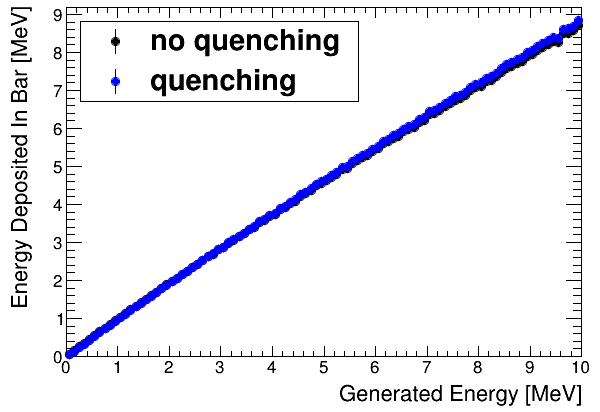
\includegraphics[width=\linewidth]{Chapter4/Figs/newQuenchPlots/e-BirksPolyQuenchingComparisonAdjusted.png}
  \captionsetup{width=.9\linewidth}
  \caption{}
  \label{subFig:electron_quenched_and_not}
\end{subfigure}%
\begin{subfigure}{.45\textwidth}
  \centering
  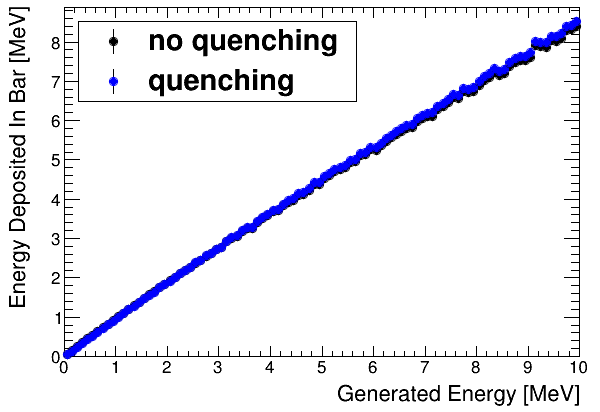
\includegraphics[width=\linewidth]{Chapter4/Figs/newQuenchPlots/e+BirksPolyQuenchingComparisonAdjusted.png}
  \captionsetup{width=.9\linewidth}
  \caption{}
  \label{subFig:positron_quenched_and_not}
\end{subfigure}
\caption{Electrons (a) and positrons (b) visible energy with and without quenching in a ``slab'' of material (see figure \ref{fig:electrons_viewed_in_slab}).}
\label{fig:electron_positron_quenched_and_not}
\end{figure}

The effect of quenching on protons is much more significant than for electrons, the charge for protons is equal and opposite to electrons but the mass is $\sim$ 2000 times greater. This results in a large amount of energy no longer being deposited in the scintillator. As the tracks are shorter but the kinetic energy still needs to be deposited resulting in larger larger $dE/dx$ values and thus more quenching as there are more ``damaged'' particles in the track. The energy deposition for both protons (see figure \ref{subFig:proton_quenched_and_not}) and anti-protons (see figure \ref{subFig:Aproton_quenched_and_not}) is linear without quenching showing that for protons and anti-protons the effect of quenching is significant. For $\alpha$ particles the effect is even more significant $\alpha$ particles which are 4 times more massive than protons but have twice the charge (see figure \ref{fig:proton_Apronton_quenched_and_not}). The loss due to quenching for protons varies from $\sim$ 90\,\% at a generated energy of 1\,MeV to $\sim$ 50\,\% at a generated energy of 10\,MeV (see figure \ref{fig:proton_Apronton_quenched_and_not}). But the effect for $\alpha$ particles is even more significant with almost none of the energy being visible below 1\,MeV and only 10\,\% of energy visible at 10\,MeV (see figure (\ref{fig:proton_Apronton_quenched_and_not})) \footnote{Visible energy is the maximum amount of energy the scintillator can produce in a given GEANT4 step given the quenching}. By looking at figures \ref{fig:electron_positron_quenched_and_not} and \ref{fig:proton_Apronton_quenched_and_not} it is easy to see the effect of quenching scaling with mass. This is the primary reason why simulating particles more massive than $\alpha$ particles is not done for VIDARR. Particles more massive than $\alpha$ particles will be quenched to such a point that they are unlikely to deposit a noticeable amount of visible energy in the detector's scintillator. 

\begin{figure}[!h]
\centering
\begin{subfigure}{.45\textwidth}
  \centering
  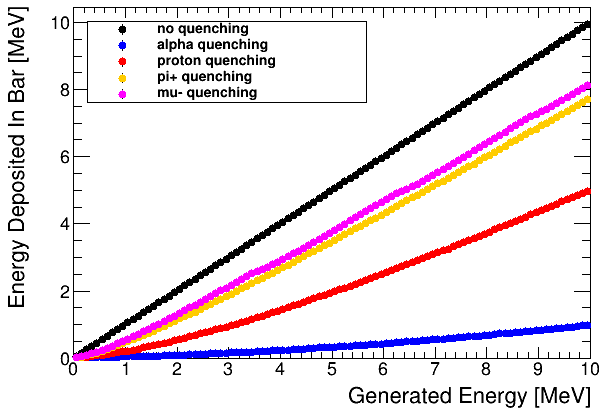
\includegraphics[width=\linewidth]{Chapter4/Figs/particleQuenchingeExample_adjusted.png}
  \captionsetup{width=.9\linewidth}
  \caption{}
  \label{subFig:proton_quenched_and_not}
\end{subfigure}%
\begin{subfigure}{.45\textwidth}
  \centering
  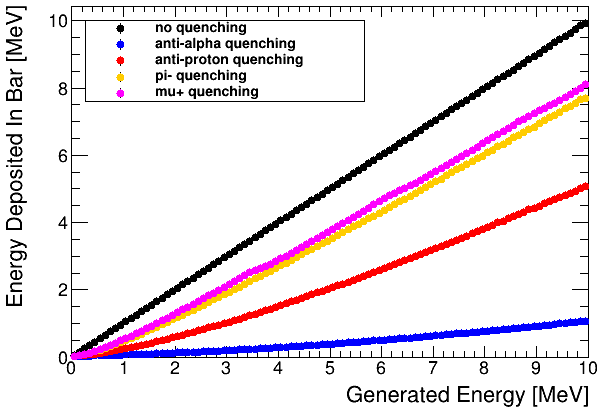
\includegraphics[width=\linewidth]{Chapter4/Figs/antiParticleQuenchingeExample_adjusted.png}
  \captionsetup{width=.9\linewidth}
  \caption{}
  \label{subFig:Aproton_quenched_and_not}
\end{subfigure}
\caption{Particles (a) and anti-particles (b) visible energy with and without quenching in a ``slab'' of material (see figure \ref{fig:electrons_viewed_in_slab}). The effect of quenching scales with the mass of the simulated particles.}
\label{fig:proton_Apronton_quenched_and_not}
\end{figure}

% \begin{figure}[!h]
% \centering
% \begin{subfigure}{.45\textwidth}
%   \centering
%   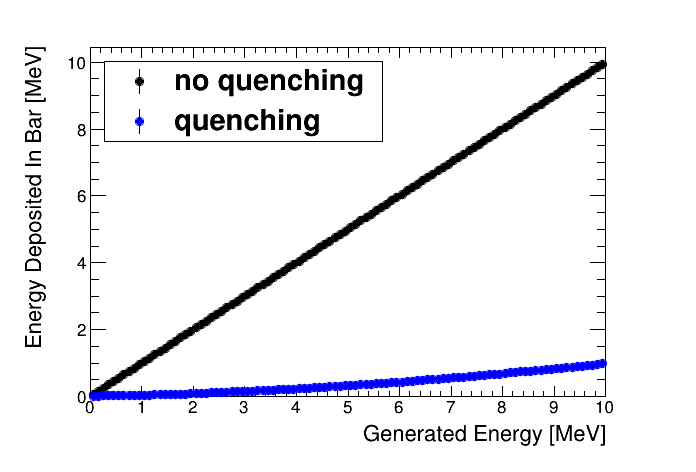
\includegraphics[width=\linewidth]{Chapter4/Figs/newQuenchPlots/alphaBirksSlab_quenchingComparison.png}
%   \captionsetup{width=.9\linewidth}
%   \caption{}
%   \label{subFig:alpha_quenched_and_not}
% \end{subfigure}%
% \begin{subfigure}{.45\textwidth}
%   \centering
%   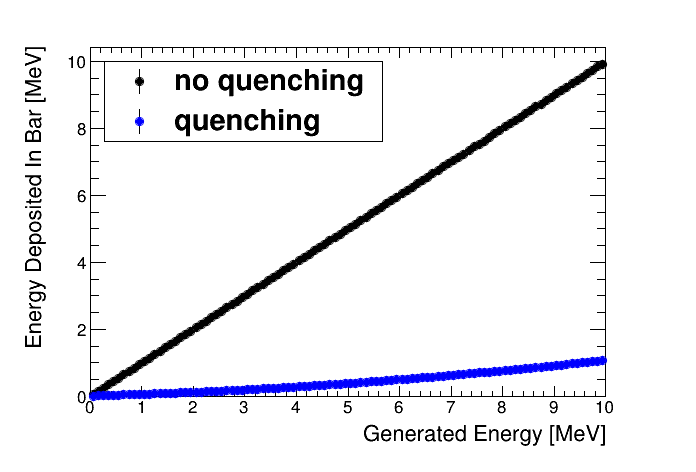
\includegraphics[width=\linewidth]{Chapter4/Figs/newQuenchPlots/aAlphaBirksSlab_quenchingComparison.png}
%   \captionsetup{width=.9\linewidth}
%   \caption{}
%   \label{subFig:Aalpha_quenched_and_not}
% \end{subfigure}
% \caption{$\alpha$ (a) and $\bar{\alpha}$ (b) particles visible energy with and without quenching in a ``slab'' of material (see figure \ref{fig:electrons_viewed_in_slab}).}
% \label{fig:alpha_Aalpha_quenched_and_not}
% \end{figure}

\section{Counting Statistics} \label{sec:GEANT4Simulation_countingStats}
When a particle passes through the scintillating medium it produces photons as it interacts with the medium. These photons then travel through the bar until they meet the WLS fibres. The photons then travel down the WLS fibres until they encounter the MPPC  this signal is then amplified by the MPPC producing a signal of 4.2\,mV per photon (in most cases) which is equivalent to one photon see figure \ref{fig:pureDarkNoise} which is called a photo-electron equivalent (PE). So for $n$ number of PE, there will be a Poisson distribution (equation \ref{equ:possionProb}) due to counting statistics. A Poisson approximation is suitable because there is a small probability of a given outcome in this case. For this distribution $pn = \overline{x}$ where $\overline{x}$ is the expectation value, substituting this into equation \ref{equ:possionProb} we get equation \ref{equ:possionExpectation} \cite{knoll_2010}.
\begin{equation}
P(x) = \frac{(pn)^x e^{-pn}}{x!}  
\label{equ:possionProb}
\end{equation}

\begin{equation}
P(x) = \frac{(\overline{x})^x e^{-\overline{x}}}{x!}  
\label{equ:possionExpectation}
\end{equation}

Further the variance of this model can be explained using equation  \ref{equ:possionVar} which also gives $\sigma^2 = \overline{x}$ giving a standard deviation of $\sigma = \sqrt{\overline{x}}$ \cite{knoll_2010}. This definition of the standard deviation is also true for the Gaussian distribution. The Gaussian distribution using this standard deviation can be seen in equation \ref{equ:guassianExpectation}. When $n$ is high enough, the Poisson distribution will approximate to a Gaussian distribution. This is useful when simulating light counting statistics because a Gaussian distribution is much less computationally intensive as there is no factorial. The tolerance for this was set to 99.9\,\% of the event in the Poisson distribution being above 2 events or more,this occurs at a mean of 10 photons. After a mean of 10 photons the Gaussian distribution is used instead. The distribution of the smearing for 10 photons can be seen in figure \ref{fig:CoutingStats10}, a slight skew in the Poisson is visible but the distributions approximate.
% The point where Gaussian is used instead of Poisson in the simulation is at a value of 10 photons seen in figure \ref{fig:CoutingStats10}. At an expectation value of 10 photons 99.9\,\% of events produced have $>$ 2 photons in the Poisson distribution (see figure \ref{fig:CoutingStats10}). This is a useful limit to switch distributions as it ensures that the low values of PE correctly modelled by the Poisson distribution are minimal. 

\begin{equation}
\sigma ^2 \equiv \sum_{x=0}^{n} (x-\overline{x})^2 P(x) = pn = \overline{x} 
\label{equ:possionVar}
\end{equation}

\begin{equation}
P(x) = \frac{1}{\sigma \sqrt[]{2 \pi}} \exp \left(-\frac{1}{2}\left(\frac{x-\overline{x}}{\sigma}\right)^{2}\right)
\label{equ:guassianExpectation}
\end{equation}

\begin{figure}[!h]
 \centering
 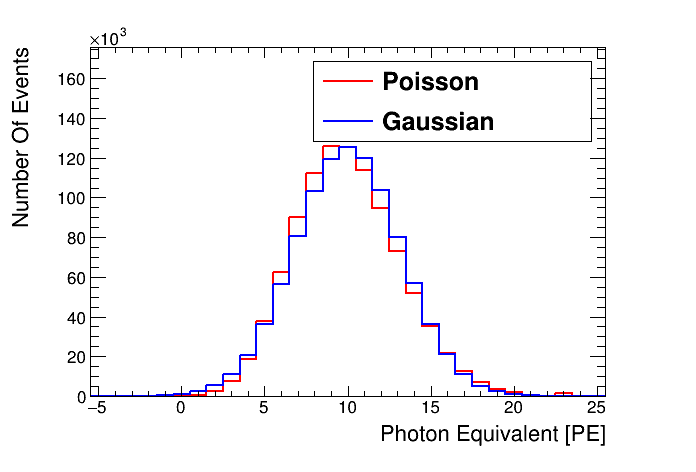
\includegraphics[width=0.7\linewidth]{Chapter4/Figs/poissionGaussian10Graph.png}
 \captionof{figure}{Counting statistics for Poisson and normal distribution for an expectation value of 10 photons the normal distribution is used when the expectation value is $\geq$ 10 photons to save on computational load.} 
 \label{fig:CoutingStats10}
\end{figure}

\section{Simulated Results With Electronics Simulation}\label{sec:GEANT4Simulation_resultsPhysicalElectronics}
The effects of quenching are mores significant for the heavier charged particles  protons, $\alpha$s and their corresponding anti-particles (see section \ref{sec:GEANT4Simulation_quenchingLoss}). The heaviest particles expected to be seen in statistically significant quantifies is the $\alpha$. Therefore, the $\alpha$ particle represents the biggest deviation from energy deposited in the scintillator and the more realistic signal expected from the detector. For this reasons $\alpha$ particles are used in this section.  
\\\\If these effects are ignored in the simulation then the results look nonphysical. In figure \ref{fig:alpha_summed_vs_truth} the summed energy inside the detector is equal to the truth energy in most cases. This is because the additional effects are being ignored and only the energy deposited in the scintillator is being reconstructed. The only events which do not have all the energy summed in the detector are those which were generated near the edges of the bar, these events are absorbed by the TiO$_2$ coating and so deposit less energy in the detector. The modelling of quenching (see section \ref{sec:GEANT4Simulation_MonteCarloBirksLaw}) and attenuation (see section \ref{sec:GEANT4Simulation_ModellingAttenuation}) therefore cause a large decrease in the summed energy inside the detector seen in figure \ref{fig:alphaVisVsTruthZoom}. Figure \ref{fig:alphaVisVsTruthZoom} is an idealistic representation of what $\alpha$ particles would look like in a VIDARR detector with perfect electronics. I.e no losses or biasing from the counting statistics (see section \ref{sec:GEANT4Simulation_countingStats}) or biasing from the MPPC PE smearing (see section \ref{sec:GEANT4Simulation_ModellingDarkNoise}).
\\\\Finally, the effects caused by the electronics (figure \ref{fig:fitting_of_non_peak_dark_noise}) and the counting statistics (figure \ref{fig:CoutingStats10}) give the simulated distribution a more realistic shape. The results for this can be seen in figure \ref{fig:alphaRecoVsTruthZoom}. With the data-driven approximations of the effects taken into account, the simulation should give a more realistic result. Unfortunately, due to the outbreak of Covid-19, the detector construction was delayed and so the accuracy of the simulation cannot be bench-marked against detector data. 


\begin{figure}[!h]
\centering
\begin{minipage}{.45\textwidth}
  \centering
  \includegraphics[width=\linewidth]{truth_vs_summed_alpha.png}
  \captionof{figure}{The energy deposited in a simulated detector by $\alpha$ particles without physical and electronic effects taken into account, this is the maximum possible energy that can be deposited.} 
  \label{fig:alpha_summed_vs_truth}
\end{minipage}%
\qquad
\begin{minipage}{.45\textwidth}
  \centering
  \includegraphics[width=\linewidth]{Chapter4/Figs/Raster/truth_vs_visSummed_alpha_zoom.png} 
  \captionof{figure}{The energy deposited in a simulated detector by $\alpha$ particles when the physical effects of quenching and attenuation are taken into account. The detector effects of dark noise and counting statistics are not taken into account}
  \label{fig:alphaVisVsTruthZoom}
\end{minipage}
\end{figure}

\begin{figure}[!h]
 \centering
 \includegraphics[width=0.5\linewidth]{Chapter4/Figs/Raster/truth_vs_recoSummed_alpha_zoom.png}
 \captionof{figure}{The energy deposited in a simulated detector by $\alpha$ particles when the physical effects of quenching and attenuation are taken into account as well as the detector effects of dark noise and counting statistics.} 
 \label{fig:alphaRecoVsTruthZoom}
\end{figure}

\section{Modelling Gadolinium}\label{sec:GEANT4Simulation_modellingGadolinium}
Gadolinium is used because of its high efficiency (10$\%$ - 40$\%$) compared to other neutron capturing materials such as $^6$Li which only has about $1\%$ \cite{Abdushukurov_2010}. The 8\,MeV $\gamma$ cascade post neutron absorption is the trigger signal for the VIDARR detector. After the cascade has been triggered the detector looks backwards in time to determine the e$^+$ cluster. The Gadolinium cascade is difficult to measure and accurately simulate for two main reasons. Firstly the Gd isotopes which have a high neutron capture cross-section are isotopes $^{155}$Gd and $^{157}$Gd \cite{molnar_2004}. Both of these nuclei are large therefore it is difficult to accurately model the individual interactions between each of the individual nucleons. There is no agreed-upon model at present for the neutron absorption onto Gadolinium and the subsequent 8\,MeV $\gamma$ cascade. The second issue is that the high energy $\gamma$-rays emitted by the cascade are very difficult to contain as they are highly penetrative. Therefore, getting accurate measurements and energy efficiencies for the cascade is also very difficult. These two problems compound one another. It is difficult to measure the cascade so it is difficult to model thus making it difficult to know what energies are expected from the Gd nucleus \cite{molnar_2004}. 
\\\\Gadolinium has two models in GEANT4 the photon evaporation model seen in figure \ref{subFig:differentGEANT4Models_photonEvaporationGd} and the final state model seen in figure \ref{subFig:differentGEANT4Models_finalStateGd}. These two models have different strengths and weaknesses the photon evaporation model conserves energy by ``boiling off'' the known decay energies of Gadolinium until there is no more energy left to disperse. This approach attempts to match the multiplicity of the gadolinium cascade but in so doing, the high energy $\gamma$-rays that are the most indicative of the gadolinium cascade are not present. The other model in GEANT4 is the final state model which tries to match the spectrum of measured energy rays. However, by using this approach the conservation of energy is violated. As the sum of the individual $\gamma$-rays exceeds the initial generated energy. Of the two models, the final state is preferred in the case of IBD. This is because the high energy $\gamma$-rays that distinguish the gadolinium cascade from the background are present in the final state model and not the photon evaporation model. Also the $\gamma$s are more likely to have the correct topology. 

\begin{figure}[!h]
\centering
\begin{subfigure}{.5\textwidth}
  \centering
  \includegraphics[width=\linewidth]{Chapter4/Figs/Raster/gadolinium/photonEvaporationGd.png}
  \captionsetup{width=.9\linewidth}
  \caption{}
  \label{subFig:differentGEANT4Models_photonEvaporationGd}
\end{subfigure}%
\begin{subfigure}{.5\textwidth}
  \centering
  \includegraphics[width=\linewidth]{Chapter4/Figs/Raster/gadolinium/FinalStateGd.png}
  \captionsetup{width=.9\linewidth}
  \caption{}
  \label{subFig:differentGEANT4Models_finalStateGd}
\end{subfigure}
\caption{Individual $\gamma$-rays for two different models for gadolinium cascade in GEANT4. The photon evaporation model conserves energy but does not produce high energy $\gamma$-rays see (a). The final state model produces high energy $\gamma$-rays but breaks the conservation of energy to do so (see (b)). Both plots from \cite{YuChen_2015}.}
\label{fig:differentGEANT4Models}
\end{figure}

%I'm not sure how useful this plot is... Natural Gadolinium is mentioned later with more context
% \begin{figure}[!h]
%  \centering
%  \includegraphics[width=0.7\linewidth]{Chapter4/Figs/Raster/gadolinium/naturalGd.png}
%  \captionof{figure}{Natural Gadolinium gamma spectra from \cite{molnar_2004}} 
%  \label{fig:naturalGd.png}
% \end{figure}

However, whilst the final state model is preferable to the photon evaporation model there is another alternative from the DANCE collaboration which produced a dicebox model of $^{157}$Gd \cite{Chyzh_2011}. DANCE is a $\gamma$ calorimeter consisting of 160 BaF$_2$ scintillation detectors. The multiplicities of the cascade from the dicebox are counted as the number of clusters that are observed rather than the number of crystals that fire in order to give a more accurate measurement of multiplicity due to the high noise rate observed in the detectors below 3\,MeV \cite{Chyzh_2011}. The shape of the spectrum at low integrated energies (below about 3\,MeV) is strongly influenced by the background from natural $\beta$ activity in the BaF$_2$ crystals, especially for low multiplicities \cite{Chyzh_2011}. Measuring the number of clusters should reduce the errors for low multiplicity according to DANCE \cite{Chyzh_2011}. The breakdown for the multiplicity cascade can be seen in figure \ref{fig:gadoliniumMultipliciesBreakdownCascade} where both the $\gamma$ and e$^-$ multiplicities are shown. Most of the multiplicities are driven by the $\gamma$-rays but some e$^-$s are produced unlike the models in GEANT4. 
\\\\The breakdown for all the energies for the DANCE dicebox is shown in figure \ref{fig:gadoliniumEnergiesCascade} where most of the energies produced are $\gamma$-rays. The dominance of the $\gamma$-rays is not surprising when comparing the dicebox to the photon evaporation and final state models in GEANT4 (figure \ref{fig:differentGEANT4Models}). The generated energies for all of the particles can be seen in figure \ref{fig:energyOfCascadeOfCascadeGd}, they resembles the photon evaporation model. The energies and particle types from figure \ref{fig:gadoliniumEnergiesCascade} are used to generate each secondary particle from the cascade. The WATCHMAN collaboration created a method to integrate the DANCE dicebox into GEANT4 by intercepting the GEANT4 function call in the ``Stacking Action'' and replace the 8\,MeV $\gamma$ cascade and forcing new secondary production via the DANCE dicebox. This implementation was copied by the VIDARR collaboration. In figure \ref{fig:energyOfCascadeOfCascadeGd} high energy $\gamma$-rays are visible unlike in the photon evaporation model (figure \ref{subFig:differentGEANT4Models_photonEvaporationGd}). However, the DANCE dicebox model also conserves energy, the total amount of energy can be seen in figure  \ref{fig:conservationOfCascadeGd}. For the DANCE dicebox, the total generated energy matches the summed energy of the particles produced in contrast to the final state model. However, the dicebox does produce less accurate $\gamma$-ray toplogy.

\begin{figure}[!h]
\centering
\begin{minipage}{.45\textwidth}
  \centering
  \includegraphics[width=\linewidth]{Chapter4/Figs/Raster/gadolinium/gadoliniumEnergiesCascade.png}
  \captionof{figure}{Energies from the DANCE dicebox based on the DANCE experimental data for $^{157}$Gd \cite{Chyzh_2011}.} 
  \label{fig:gadoliniumEnergiesCascade}
\end{minipage}%
\qquad
\begin{minipage}{.45\textwidth}
  \centering
  \includegraphics[width=\linewidth]{Chapter4/Figs/Raster/gadolinium/gadoliniumMultipliciesBreakdownCascade.png} 
  \captionof{figure}{Multiplicities from the DANCE dicebox based on the DANCE experimental data for $^{157}$Gd \cite{Chyzh_2011}. }
  \label{fig:gadoliniumMultipliciesBreakdownCascade}
\end{minipage}
\end{figure}

% \begin{figure}[!h]
%  \centering
%  \includegraphics[width=0.7\linewidth]{Chapter4/Figs/Raster/gadolinium/pe_vs_fs_models_summed.png}
%  \captionof{figure}{blah.} 
%  \label{fig:pe_vs_fs_models_summed}
% \end{figure}

\begin{figure}[!h]
\centering
\begin{minipage}{.45\textwidth}
  \centering
  \includegraphics[width=\linewidth]{Chapter4/Figs/Raster/gadolinium/energyOfCascadeOfCascadeGd.png}
  \captionof{figure}{Energy of all particles from the $^{157}$Gd dicebox based on the DANCE experiment \cite{Chyzh_2011} which is then worked into GEANT4 using an implementation created by the WATCHMAN collaboration which was then copied by the VIDARR collaboration.} 
  \label{fig:energyOfCascadeOfCascadeGd}
\end{minipage}%
\qquad
\begin{minipage}{.45\textwidth}
  \centering
  \includegraphics[width=\linewidth]{Chapter4/Figs/Raster/gadolinium/conservationOfCascadeGd.png} 
  \captionof{figure}{The summed energy for the Dicebox gadolinium $\gamma$ cascade. There is no violation of the conservation of energy 8\,MeV energy is generated and 8\,MeV is observed by the simulation.}
  \label{fig:conservationOfCascadeGd}
\end{minipage}
\end{figure}

The photon evaporation model and final state model were overlapped with the measured spectrum from natural gadolinium as well as $^{155}$Gd,$^{157}$Gd in figure \ref{fig:comparisonGd}. The high energy $\gamma$-rays observed in the natural and specific isotopes of Gd are present in the final state model which reads from the database ENDF \cite{BROWN20181} and tries to replicate the final state of the neutron \cite{koiTatsumi_2006}. With the final state model events in the low energy tail break Q-value (conservation of energy) \cite{YuChen_2015}. By taking figure \ref{fig:comparisonGd} and overlaying the DANCE/WATCHMAN dicebox (figure \ref{fig:comparisonAndDiceBoxGd}) the similarities between photon evaporation model and dicebox are clear but it extends further producing more higher energy $\gamma$-ray. The dicebox shown in figure \ref{fig:comparisonAndDiceBoxGd} only represents $^{157}$Gd. The DANCE dicebox was based on data measured from a sample that was  99.7\,\% $^{157}$Gd \cite{Chyzh_2011}. 

\begin{figure}[!h]
 \centering
 \includegraphics[width=0.7\linewidth]{Chapter4/Figs/Raster/gadolinium/comparisonGd.png}
 \captionof{figure}{How the photon evaporation and final state models in GEANT 4 compare to the measured spectra for natural gadolinium and Gd 155,157. High energy $\gamma$s are only present in the final state model.  * \cite{kandlakunta_2012} ** \cite{bollinger_1970} from \cite{YuChen_2015}.} 
 \label{fig:comparisonGd}
\end{figure}

\begin{figure}[!h]
 \centering
 \includegraphics[width=0.7\linewidth]{Chapter4/Figs/Raster/gadolinium/comparisonAndDiceBoxGd.png}
 \captionof{figure}{Figure \ref{fig:comparisonGd} \cite{YuChen_2015} but with the Dicebox individual $\gamma$-rays for $^{157}$Gd from figure \ref{fig:energyOfCascadeOfCascadeGd} overlaid on top. The Dicebox has similar low energy $\gamma$-rays to the photon evaporation model but has more high energy $\gamma$-rays as would be expected of the Gd cascade. * \cite{kandlakunta_2012} ** \cite{bollinger_1970}.}
 \label{fig:comparisonAndDiceBoxGd}
\end{figure}

The energies of the $\gamma$-rays produced by the simulation are shown in figure \ref{fig:gdCascadeVsAllGammas}. The gadolinium cascade is from a simulation of natural gadolinium which uses the DANCE/WATCHMAN dicebox when $^{157}$Gd captures a neutron and uses the final state model when other isotopes of Gd capture a neutron. In figure \ref{fig:gdCascadeVsAllGammas} the majority of the $\gamma$-rays produced are from the $^{157}$Gd dicebox final state model hybrid. However, there is also a significant peak caused by the hydrogen neutron capture. The effect of adding the dicebox to the final state model can be seen in figure \ref{fig:TotalGeneratedEnergyOfCascadeFinalStateDicebox}. Compared to the final state model the peaks in the dicebox final state hybrid are much more pronounced with more energy being produced overall. The focus on the high energy $\gamma$-rays also means that more energy is deposited in the scintillator as well (figure \ref{fig:finalStateAndDiceBoxBarsDepositedEnergy}). This is very useful for the VIDARR simulation, not only is the dicebox-final state hybrid more realistic than the pure final state model it also shows that the trigger signal for the VIDARR detector is even more unique than expected. When comparing the dicebox to the final state model the dicebox deposits more energy in the scintillator than would be expected from the pure final state model (figure \ref{fig:finalStateAndDiceBoxBarsDepositedEnergy}) and also hits more bars as seen in figure \ref{fig:numberOfBarsHitCascadeFinalStateDicebox}. This is especially useful for separating out the trigger signal from the noise as will be shown in section \ref{sec:MachineLearningTrigger}.

\begin{figure}[!h]
\centering
\begin{minipage}{.45\textwidth}
  \centering
  \includegraphics[width=\linewidth]{Chapter4/Figs/Raster/gadolinium/gdCascadeVsAllGammas.png}
  \captionof{figure}{The individual $\gamma$-rays seen in the simulated VIDARR detector from generated neutrons with 0.025\,eV kinetic energy. The majority of the distribution is dominated by gadolinium cascade but a small peak is caused by the hydrogen absorption of the neutron.} 
  \label{fig:gdCascadeVsAllGammas}
\end{minipage}%
\qquad
\begin{minipage}{.45\textwidth}
  \centering
  \includegraphics[width=\linewidth]{Chapter4/Figs/Raster/finalStateAndDiceBoxBarsGeneratedEnergy.png} 
  \captionof{figure}{Total generated energy of the cascade the dicebox based on the DANCE detector data \cite{Chyzh_2011}. When replacing the $^{157}$Gd final state interaction with the dicebox more energy is generated.}
  \label{fig:TotalGeneratedEnergyOfCascadeFinalStateDicebox}
\end{minipage}
\end{figure}

\begin{figure}[!h]
\centering
\begin{minipage}{.45\textwidth}
  \centering
  \includegraphics[width=\linewidth]{Chapter4/Figs/Raster/finalStateAndDiceBoxBarsDepositedEnergy.png}
  \captionof{figure}{The total energy deposited in the simulated VIDARR detector. Slightly more energy is deposited by the final state + Dicebox model. (0th bin for Final state No $^{157}$Gd goes up to 80000)} 
  \label{fig:finalStateAndDiceBoxBarsDepositedEnergy}
\end{minipage}%
\qquad
\begin{minipage}{.45\textwidth}
  \centering
  \includegraphics[width=\linewidth]{Chapter4/Figs/Raster/finalStateAndDiceBoxBarsHit.png} 
  \captionof{figure}{The number of bars hit in the simulated VIDARR detector for different models. The final state model with the dicebox $^{157}$Gd was chosen and hits slightly more bars.}
  \label{fig:numberOfBarsHitCascadeFinalStateDicebox}
\end{minipage}
\end{figure}

\section{Machine Learning Neutron Trigger}\label{sec:MachineLearningTrigger}
There are several machine learning techniques available to analyse different types of data. Typically the physics field uses decision trees (DT), k-nearest neighbours (knn), and deep learning neural networks (DLNN). One technique which is often neglected is the support vector machine (SVM) \cite{Boser92atraining}, \cite{cortes1995support}. An SVM is a linear classifier that uses particular points (support vectors) in two data sets to find the best separating ``hyperplane'' an n-dimensional line that finds the maximum separation between the two data sets (see figure \ref{fig:svmBoser92LinearSVM}). Whilst the SVM is a linear classifier it is possible to use a function to distort non-lienar data such that it becomes linearly separable. Theses functions are called kernels an example of how they are used can be seen in figure \ref{fig:kernelRBF_fromWeB}. The kernel used in figure \ref{fig:kernelRBF_fromWeB} is the radial bas function (RBF) kernel described by equation \ref{equ:RbfKernelFunc}. The method of tranforming data through a kernel via the ``kernel trick'' is well established and has been a common technique since at least 1992 \cite{Boser92atraining}.
% Using simulated data it is possible to test whether a machine learning trigger would be advantageous to the analysis. The machine learning technique considered the most appropriate was the Support Vector Machine (SVM) \cite{Boser92atraining} \cite{cortes1995support}, as SVMs were compared to several other simple techniques typically used in physics namely a decision tree and k-nearest neighbours (see figure \ref{fig:sklearnReleventExamples}). As seen in figure \ref{fig:sklearnReleventExamples} the SVM linearly or with a kernel. The radial basis function (RBF) kernel is one of the most common. In figure \ref{fig:sklearnReleventExamples} the generalised boundaries, high accuracy, and well-defined projection space seen in the RBF SVM make it the clear standout. The SVM utilises the RBF kernel via the kernel trick since at least 1992 \cite{Boser92atraining}. 
% \\\\SVMs work by finding the best separating hyperplane between two opposing data sets. In figure \ref{fig:svmBoser92LinearSVM} the best separating hyperplane is calculated for a simple data set. The SVM works by finding the maximum distance between each data set and creating an n-dimensional line the ``hyperplane'' to separate the data. In order to separate non-linear data the kernel trick is used which figure \ref{fig:kernelRBF_fromWeB} shows. Figure \ref{fig:kernelRBF_fromWeB} also shows how two different kernels achieve the same result. How the decision surface is manipulated to separate data sets is shown in figure \ref{fig:kernelRBF_fromWeB}. As figure \ref{fig:kernelRBF_fromWeB} shows the kernel transforms the data set so it becomes linearly separable for the SVM. A further test of the SVMS's capabilities is done in figure \ref{fig:svmExp_GausseExamples} which tests the separation of multiple Gaussian data sets from 2D exponential noise. This is as complex ass trigger data could reasonably be expected to be. This means that the SVM should be suitable for separating neutron trigger data. 
% \\\\An SVM is also convexly optimised which means the solutions are easier to solve as there is only one global minimum \cite{cortes1995support}. This feature allows SVMs to train on sparse data sets with low statistics. SVMs are fast to train on small data sets but as data sets grow larger the squared nature of the SVM solution increases training times dramatically \cite{cortes1995support}. This means that for data with many dimensions and many statistics training times and memory usage can be very high to the point of being unusable \cite{cortes1995support}. Data must also be completely labelled and optimisation for training whilst possible through sequential minimal optimisation is somewhat limited \cite{platt1998sequential}. These drawbacks are not a significant issue for the trigger data but they should be bared in mind for more complex cases such as image recognition.
\begin{equation}
K(\mathbf{x,x'}) = \exp{(\gamma \mathbf{x \cdot x'})} - 1
\label{equ:RbfKernelFunc}
\end{equation}

\begin{figure}[!h]
\centering
\includegraphics[width=0.9\linewidth]{Chapter4/Figs/Raster/svmLinAndRbf/svmBoser92LinearSVM.png}
\captionof{figure}{An example of how a support vector machine (SVM) separates two different distributions that are linearly separable. The maths behind the classifier finds the best separating line/hyper-plane between two distributions. From \cite{Boser92atraining}.} 
\label{fig:svmBoser92LinearSVM}
\end{figure}

% \begin{figure}[!h]
% \centering
% \includegraphics[width=0.7\linewidth]{Chapter4/Figs/Raster/svmLinAndRbf/svmBoser92KernelSVM.png}
% \captionof{figure}{How a support vector machine (SVM) operates with a kernel being applied using a squared polynomial kernel on the left and a radial basis function (RBF) on the right. By using the ``kernel trick'' it is possible to separate non-linear data. From \cite{Boser92atraining}.} 
% \label{fig:svmBoser92KernelSVM}
% \end{figure}

\begin{figure}[!h]
\centering
\includegraphics[width=0.9\linewidth]{Chapter4/Figs/Raster/svmLinAndRbf/kernelRBF_fromWeB.png}
\captionof{figure}{An online example that shows how the kernel trick is used to make non-linear data linearly separable by transforming it through a kernel. From \cite{kernelTrickWeb}.} 
\label{fig:kernelRBF_fromWeB}
\end{figure}
 
A direct comparison between DT, knn, linear (no kernel) SVM and RBF SVM classifiers is done in figure \ref{fig:sklearnReleventExamples}. In figure \ref{fig:sklearnReleventExamples} the generalised boundaries, high accuracy and well defined projection space of the RBF SVM make it the clear standout. However, each machine learning technique has its drawbacks. Whilst SVMs are convexly optimised only having one global minimum \cite{Boser92atraining} (see figures \ref{fig:svmBoser92LinearSVM} and \ref{fig:sklearnReleventExamples}) this comes at the cost of Parallelisation. In order to achieve the well defined projection space with such a simple algorithm the SVM must be able to observe the whole of the data at once. his is somewhat mitigated by sequential minimal optimisation \cite{platt1998sequential} but not completely. This means that for very large data sets with thousands of dimensions an SVM might not always be suitable as training times become too long. However, the trigger data for the VIDARR detector only has a maximum of 4 dimensions shown in table \ref{tab:triggerDims}. Data must also be labelled for SVMs as well but this is not a significant limitation for VIDARR data sets, as labelling of data is likely to be done regardless of machine learning.
 
\begin{figure}[!h]
\centering
\includegraphics[width=\linewidth]{Chapter4/Figs/Raster/svmLinAndRbf/sklearnReleventExamples.png}
\captionof{figure}{Some example classifiers taken from scikit-learn that show how different techniques draw boundaries and how confident they are in those boundaries. Decision trees and k nearest neighbours are common simplistic classifiers used in physics but the boundaries they produce are often susceptible to over-training. The linear SVM is generalised but is quite limited in its utility. The SVM with the RBF kernel consistently draws the most accurate boundaries and they are well generalised. The accuracy of each technique is shown in the bottom right of each plot. From \cite{scikit-learn}.} 
\label{fig:sklearnReleventExamples}
\end{figure}

\begin{table*}[!h]
\centering
\begin{tabular}{lll}  
\toprule
Dimension               & Th 1.5\,PE (0.06\,MeV) & Th 12.5\,PE (0.5\,MeV)\\
\midrule
\# of Bars Hit Above Th &  NBATh$_{1.5}$         & NBATh$_{12.5}$\\
Summed Energy Above Th  &  SEATh$_{1.5}$         & SEATh$_{12.5}$\\
\bottomrule  
\end{tabular}
\caption{A table showing the 4 dimensions that the trigger can have. The word threshold is abbreviated to Th for convenience.}
\label{tab:triggerDims}
\end{table*}

%Nyström
% Figures \ref{fig:sklearnReleventExamples} \ref{fig:svmBoser92LinearSVM} \ref{fig:kernelRBF_fromWeB} \ref{fig:kernelRBF_fromWeB} \ref{fig:svmExp_GausseExamples} are sufficient reason to believe that an SVM with an RBF kernel should be a suitable classifier for separating trigger data that only has four dimensions. The four dimensions that need to be optimised are: the summed energy above a threshold of 1.5\,PE (0.06\,MeV), summed energy above a threshold of 12.5\,PE (0.5\,MeV), Numbers of bars hit above a threshold of 1.5\,PE (0.06\,MeV), Numbers of bars hit above threshold 12.5\,PE (0.5\,MeV). The libraries used were LIBSVM and LIBLINEAR both of which are highly provident and often cited as the reason for the SVMs gain in popularity \cite{chang2011libsvm} \cite{fan2008liblinear} \cite{murty2016support}. The wrapper in sci-kit learn was the preferred method due to its ease of use and its convenient application of the Nystrom approximation \cite{williams2001using} of the kernel. The Nystroem approximation is useful as the amount of computation required for a complete kernel SVMs scales $\sim$ O (n$^3$) where n is the number of training examples \cite{williams2001using}. By using a sample of size m to compute an approximation of the kernel the amount of computation required scales $\sim$ O (m$^2$n) instead \cite{williams2001using}. This approach will work even when m $\ll$ n \cite{williams2001using}. The example data shown in figure \ref{fig:svmExp_GausseExamples} shows how LIBLINEAR when combined with with an RBF Nystroem approximated kernel performs in comparison to LIBSVM with a complete RBF kernel the boundaries are very similar. From this point, the LIBLINEAR library and the Nystroem approximation will be used to speed up training and to prevent memory overflow which can happen when the SVM isn't converging and when large data sets are used. The simulated data set has 1 million neutron signal events and 4 million background events.

There is also another issue when using a kernel SVM, the kernel itself greatly increase computational requirement. A linear (no kernel) SVM requires computational power that scales O $\sim$ n$^2$ (where n is the number of training samples) \cite{cortes1995support}. But when a kernel is used the computational power required scales with O $\sim$ n$^3$ instead \cite{williams2001using}. In order to mitigate this an approximate kernel is created via the Nyström method. By using a sample size of m to cmopute this approximate kernel the computation requirement scales with O $\sim$ mn$^2$ \cite{williams2001using}. This approach will work effectively even when m << n \cite{williams2001using}. 
\\\\Due to it's preexisting implementation of the Nyström kernel approximation the wrapper scikit-learn was chosen as it saved development time \cite{scikit-learn}. Scikit-learn uses LIBSVM \cite{chang2011libsvm} and LIBLINEAR \cite{fan2008liblinear} both of which are highly provident and often cited as the reason for the SVM's gain in popularity \cite{murty2016support}. In figure \ref{fig:svmExp_GausseExamples} a non-linear data set with two Gaussian signal distributions and an exponential distribution in (x,y) for noise is separated with LIBSVM using an RBF kernel (figure \ref{subFig:svmExp_2GausseExample}) and LIBLINEAR using an approximated Nyström kernel (figure \ref{subFig:exp_2NysGaussExample}). The example data shown in figure \ref{fig:svmExp_GausseExamples} shows how LIBLINEAR when combined with a Nyström approximated kernel performs to a similar standard to LIBSVM with a full RBF kernel, the boundaries are extremely similar. It also shows that scikit-learn's implementation of the Nyström method is quite accurate and can be trusted. From this point the LIBLINEAR library and the Nyström approximated RBF kernel will be used to speed up training and prevent an excess use of computational resource. Considering the strengths of SVMs, the low dimensionality of the trigger data, and the effective use of available computational resource the approximate RBF SVM should be more than sufficient for separating out the 1 million generated signal events and the 4 million generated background events. 

\begin{figure}[!h]
\centering
\begin{subfigure}{.5\textwidth}
  \centering
  \includegraphics[width=\linewidth]{Chapter4/Figs/adjustedSvmPlots/adjusted_exp_2GaussExample.png}
  \captionsetup{width=.9\linewidth}
  \caption{}
  \label{subFig:svmExp_2GausseExample}
\end{subfigure}%
\begin{subfigure}{.5\textwidth}
  \centering
  \includegraphics[width=\linewidth]{Chapter4/Figs/adjustedSvmPlots/adjusted_exp_2NysGaussExample.png}
  \captionsetup{width=.9\linewidth}
  \caption{}
  \label{subFig:exp_2NysGaussExample}
\end{subfigure}
\caption{SVM examples showing how to separate data sets with two Gaussian signals (blue) from exponential noise (red). For both an RBF kernel was used with c = 10$^4$ and $\gamma$ = 1. In (a) LIBSVM is used with an RBF kernel and support vectors are highlighted in orange. In (b) LIBLINEAR is used with a Nyström approximation of the RBF kernel with a sampling (m) of 100.}
\label{fig:svmExp_GausseExamples}
\end{figure}

Kernel SVMs have two factors that can be tuned to give more accurate results. The soft margin C, and $\gamma$ which is part of the RBF kernel described by equation \ref{equ:RbfKernelFunc} \cite{Boser92atraining}. Higher values of C correspond to a lower amount of signal and noise overlap and vice versa \cite{cortes1995support}. Typically C can vary from 10$^{-6}$ to 10$^6$ but can be even higher or even lower providing its $>$ 0. Values for $\gamma$ must also be $>$ 0 and will vary depending on the linearity of the data. For an example of what non-linear data looks like when searching for suitable C and $\gamma$ values figure w\ref{fig:GammaCGridSearchExp2Gauss} was produced which shows how the values for figure \ref{subFig:exp_2NysGaussExample} where chosen. A higher value of $\gamma$ corresponds to higher non-linearity. With this information, we can see that there is some overlap in figure \ref{subFig:exp_2NysGaussExample} and is very non-linear so this search for relevant C and $\gamma$ values corroborates what can be seen in the example data. In contrast, the generated neutron and noise data shows clear linearity as a low $\gamma$ value of 1 is preferred and has a small overlap as a high C value of 10$^6$ is preferred (see figure \ref{fig:GammaCGridSearchNeutron}). This shows that the generated neutron data is very easy to separate with a linear classifier and so using anything more complex than an SVM would be unlikely to yield better results.

\begin{figure}[!h]
\centering
\begin{minipage}{.45\textwidth}
  \centering
  \includegraphics[width=\linewidth]{Chapter4/Figs/Raster/GammaCGridSearchExp2Gauss_adjust.png}
  \captionof{figure}{SVMs being trained on varying values of C and $\gamma$ for figure \ref{subFig:exp_2NysGaussExample}. Higher values of $\gamma$ represent non-linear data separation which the SVMs settle on. Higher values of C represent more overlap in the data. C choice is less clear but ultimately a higher value of C was settled due to a high preference for isolating boundaries as much as possible. A $\gamma$ = 1 and C of 10$^4$ was chosen.} 
  \label{fig:GammaCGridSearchExp2Gauss}
\end{minipage}%
\qquad
\begin{minipage}{.45\textwidth}
  \centering
  \includegraphics[width=\linewidth]{Chapter4/Figs/Raster/GammaCGridSearchNeutron_adjust.png}
  \captionof{figure}{SVMs being trained on varying values of C and $\gamma$ for figure generated background and neutron data. Lower values of $\gamma$ represent a linear data separation which the SVMs settle on. Higher values of C represent more overlap in the data. This data set is linearly separable with minimal overlap. A $\gamma$ = 10$^{-6}$ and C of 10$^6$ was chosen.}
  \label{fig:GammaCGridSearchNeutron}
\end{minipage}
\end{figure}

%NBATh$_{1.5}$ & NBATh$_{12.5}$ SEATh$_{1.5}$ & SEATh$_{12.5}$\\
Once C and $\gamma$ have been chosen a basic form of dimensional reduction was done to assess the impact each dimension has on the classifier (see figure \ref{fig:accNeutronSVMC1e6_g1e-6}). In figure \ref{fig:accNeutronSVMC1e6_g1e-6} the addition of more dimensions beyond 2 does not seem to increase accuracy suggesting that not all of the information provided by the emulated trigger is useful. This is also true for the efficiency as seen in figure \ref{fig:effNeutronSVMC1e6_g1e-6} and the purity as seen in figure \ref{fig:purNeutronSVMC1e6_g1e-6}. This shows that not only is the data linearly separable, it is actually 2d linearly separable, meaning it is extremely easy for any machine learning algorithm to separate. Let alone one as powerful as the RBF SVM, this technique is overkill for this particular data set, hence why a DLNN has not been pursued for this data set. The most accurate would be the SEATh$_{1.5}$ + NBATh$_{1.5}$. However, the option: NBATh$_{1.5}$ + NBATh$_{12.5}$ is eassier to implement for the electronics on VIDARR. The drop in accuracy, efficiency, and purity is relatively low for this combination and therefore it is the preferred option. 

\begin{figure}[!h]
\centering
\includegraphics[width=0.8\linewidth]{Chapter4/Figs/Raster/accNeutronSVMC1e6_g1e-6.png}
\captionof{figure}{Accuracy for Nyström SVM classifiers with approximate RBF kernel with a sample of 100 for generated neutron and noise data. With C = 10$^6$ and $\gamma$ = 10$^{-6}$. Separation doesn't improve above 2 dimensions.} 
\label{fig:accNeutronSVMC1e6_g1e-6}
\end{figure}

\begin{figure}[!h]
\centering
\begin{minipage}{.45\textwidth}
  \centering
  \includegraphics[width=\linewidth]{Chapter4/Figs/Raster/effCombSVMAdjust.png}
  \captionof{figure}{Efficiency for Nyström SVM classifiers with approximate RBF kernel with a sample of 100 for generated neutron and noise data. With C = 10$^6$ and $\gamma$ = 10$^{-6}$. Separation doesn't improve above 2 dimensions.} 
  \label{fig:effNeutronSVMC1e6_g1e-6}
\end{minipage}%
\qquad
\begin{minipage}{.45\textwidth}
  \centering
  \includegraphics[width=\linewidth]{Chapter4/Figs/Raster/purCombSVMAdjust.png}
  \captionof{figure}{Purity for Nyström SVM classifiers with approximate RBF kernel with a sample of 100 for generated neutron and noise data. With C = 10$^6$ and $\gamma$ = 10$^{-6}$. Separation doesn't improve above 2 dimensions.}
  \label{fig:purNeutronSVMC1e6_g1e-6}
\end{minipage}
\end{figure}

The chosen classifier is seen in figure \ref{fig:signalAndNoiseNeutronSVM_C1e6_g1e-6}, which as figure \ref{fig:purNeutronSVMC1e6_g1e-6} indicates is a linear classifier with minimal overlap between the signal noise. In figure \ref{fig:signalAndNoiseNeutronSVM_C1e6_g1e-6} anything to the left of the line is considered a noise event and anything to the right of the line is considered a neutron event. The effect of this selection criteria can be seen in figure \ref{fig:summedEnergyPastTriggerGdDicebox} which shows the summed energy that makes it past the emulated trigger. The amount of summed energy past the emulated trigger is overwhelmingly dominated by the 8\,MeV $\gamma$ cascade from the neutron absorption. The only events that are able to make it past the emulated trigger are the electrons with high generated kinetic energies (past $\sim$ 4\,MeV) as seen in figure \ref{fig:GeneratedEnergyPastTriggerGdDicebox} but they are unlikely to be present when in sufficient quantities when the detector is deployed. 

\begin{figure}[!h]
\centering
\begin{subfigure}{.5\textwidth}
  \centering
  \includegraphics[width=\linewidth]{Chapter4/Figs/Raster/noiseNeutronSVM_C1e6_g1e-6.png}
  \captionsetup{width=.9\linewidth}
  \caption{}
  \label{subFig:noiseNeutronSVM_C1e6_g1e-6}
\end{subfigure}%
\begin{subfigure}{.5\textwidth}
  \centering
  \includegraphics[width=\linewidth]{Chapter4/Figs/Raster/signalNeutronSVM_C1e6_g1e-6.png}
  \captionsetup{width=.9\linewidth}
  \caption{}
  \label{subFig:signalNeutronSVM_C1e6_g1e-6}
\end{subfigure}
\caption{A 2d SVM classifier trained on signal and noise data with the number of bars hit above 1.5\,PE (0.06\,MeV) and the number of bars hit above 12.5\,PE (0.5\,MeV) with a Nystrom approximate RBF kernel with a sampling of 100, C value of 10$^6$ and $\gamma$ value of 10$^{-6}$. The generated noise is seen in (a) the generated signal (neutron induced Gd cascade) is shown in (b). Support vectors are shown by the dashed lines. The decision boundary is shown by the solid line.}
\label{fig:signalAndNoiseNeutronSVM_C1e6_g1e-6}
\end{figure}

\begin{figure}[!h]
\centering
\begin{minipage}{.45\textwidth}
  \centering
  \includegraphics[width=\linewidth]{Chapter4/Figs/Raster/gadolinium/summedEnergyPastTriggerGdDicebox.png}
  \captionof{figure}{The summed energy of the neutron events that survive past the trigger. The simulated neutron trigger shown in figure \ref{fig:signalAndNoiseNeutronSVM_C1e6_g1e-6}. 25\,PE = 1\,MeV overall giving an Efficiency = 75.6\,\% and purity = 93.5\,\%. Purity is determined from a background of 4 million noise events and 1 million signal events.} 
  \label{fig:summedEnergyPastTriggerGdDicebox}
\end{minipage}%
\qquad
\begin{minipage}{.45\textwidth}
  \centering
  \includegraphics[width=\linewidth]{Chapter4/Figs/Raster/gadolinium/GeneratedEnergyPastTriggerGdDicebox.png}
  \captionof{figure}{The generated kinetic energy for particles which make it past the simulated neutron trigger. The only particles of concern are electrons that produce high enough energy to hit many bars and produce showers. Background electrons with energies > $\sim$4\,MeV are unlikely to be prevalent during deployment.}
  \label{fig:GeneratedEnergyPastTriggerGdDicebox}
\end{minipage}
\end{figure}

\clearpage
These results show two points. The fist is that the RBF SVM is significantly more capable than required for separating the trigger data. The seconds is that the VIDARR trigger should be very effective at distinguishing the $\gamma$ cascade from background expected at reactor sites. This is highly encouraging as it indicates that VIDARR's segmentation and technology are well suited to resolving the trigger signal from noise. It is possible that smaller segmentation will yield better results but considering the high simulated efficiency (75.6\,\%) it is unlikely to improve significantly. As a result, it can be concluded that VIDARRR's segmentation is in a ``sweet spot'' where the signal is easy to separate whilst retaining relevant information. So much so that machine learning cannot improve upon it. This conclusion will also be reinforced by the cosmic $\mu$ tomography results in chapter \ref{chp:cosmicMuonTomography}.

% \begin{figure}[!h]
%  \centering
%  \includegraphics[width=0.7\linewidth]{Chapter4/Figs/Raster/gadolinium/summedEnergyPastTriggerGdDicebox.png}
%  \captionof{figure}{} 
%  \label{fig:summedEnergyPastTriggerGdDicebox}
% \end{figure}

% \begin{figure}[!h]
%  \centering
%  \includegraphics[width=0.7\linewidth]{Chapter4/Figs/Raster/gadolinium/GeneratedEnergyPastTriggerGdDicebox.png}
%  \captionof{figure}{} 
%  \label{fig:GeneratedEnergyPastTriggerGdDicebox}
% \end{figure}

%*******************************************************************************
%***************************************  End  *********************************
%*******************************************************************************